\documentclass{article}
\usepackage[utf8]{inputenc}
\usepackage[sexy]{evan}

\usepackage[english]{babel}
\usepackage{graphicx}
\usepackage{float}

\begin{document}

\begin{titlepage}

\newcommand{\HRule}{\rule{\linewidth}{0.5mm}} % Defines a new command for the horizontal lines, change thickness here

\center % Center everything on the page
 
%----------------------------------------------------------------------------------------
%	HEADING SECTIONS
%----------------------------------------------------------------------------------------

\textsc{\LARGE Northwestern University}\\[1.5cm] % Name of your university/college
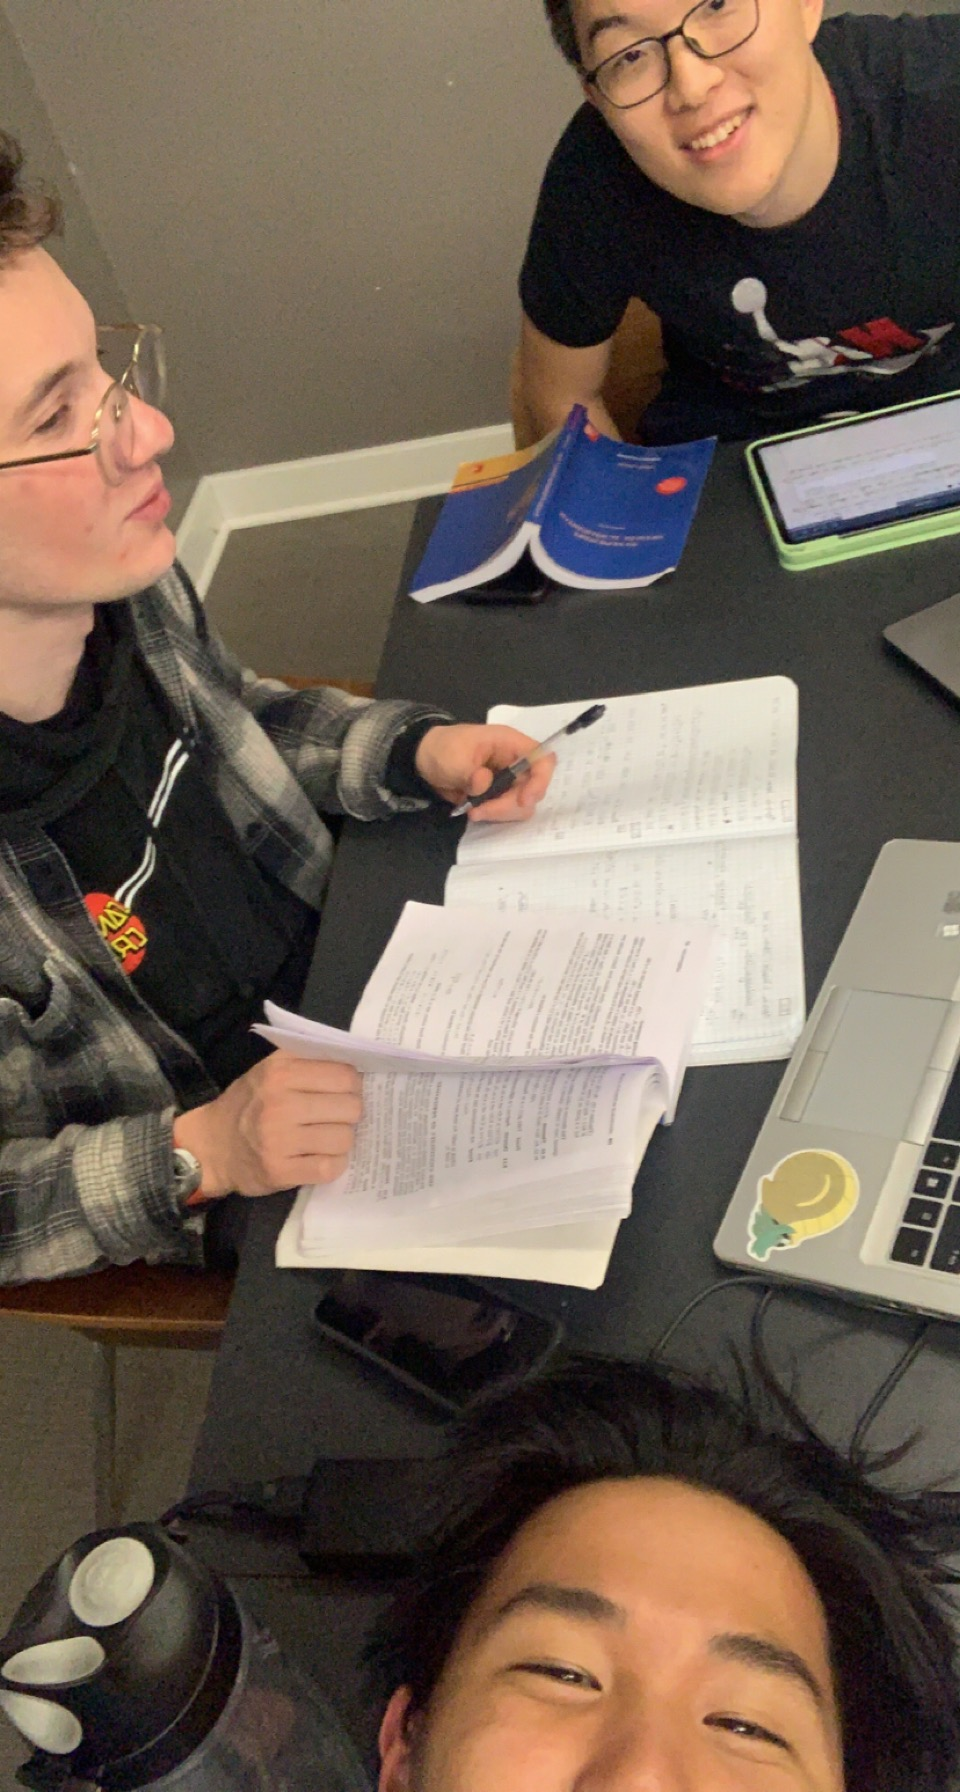
\includegraphics[scale=.1]{IMG_6914.JPG}\\[2cm] % Include a department/university logo - this will require the graphicx package
\textsc{\Large Real Analysis}\\[0.5cm] % Major heading such as course name
\textsc{\large MATH 321-1}\\[0.5cm] % Minor heading such as course title

%----------------------------------------------------------------------------------------
%	TITLE SECTION
%----------------------------------------------------------------------------------------

\HRule \\[0.4cm]
{ \huge \bfseries theorems! definitions! examples!}\\[0.4cm] % Title of your document
\HRule \\[1.5cm]
 
%----------------------------------------------------------------------------------------
%	AUTHOR SECTION
%----------------------------------------------------------------------------------------

\begin{minipage}{0.4\textwidth}
\begin{flushleft} \large
\emph{Author:}\\
Elliott \textsc{Yoon}\\ % Your name
\end{flushleft}

\end{minipage}\\[2cm]

% If you don't want a supervisor, uncomment the two lines below and remove the section above
%\Large \emph{Author:}\\
%John \textsc{Smith}\\[3cm] % Your name

%----------------------------------------------------------------------------------------
%	DATE SECTION
%----------------------------------------------------------------------------------------

{\large \today}\\[2cm] % Date, change the \today to a set date if you want to be precise

\vfill % Fill the rest of the page with whitespace

\end{titlepage}

\section{The Real and Complex Numbers}
\prototype{$\RR$ is an ordered field with the least-upper-bound property and subfield $\QQ$.}
\begin{definition}
    Let $S$ be any set.
    \begin{itemize}
        \ii If $x$ is a member of $S$, we write $x\in S$. Otherwise, we write $x\not\in S$.
        \ii The set without any elements is called the \vocab{empty set}, often written as $\emptyset$.
        \ii If $A$ and $B$ are sets and every element of $A$ is an element of $B$, we say that $A$ is a \emph{subset} of $B$ and write $A\subset B$ or $B\supset A$. 
        \ii If $A\subset B$ and $B\subset A$, we write $A=B$.
    \end{itemize}   
\end{definition}

\begin{definition}
    Let $S$ be a set. An \vocab{order} on $S$ is a relation, $<$, with the following two properties:
    \begin{enumerate}
        \item If $x,y\in S$, then \emph{exactly} one of the statements is true:
        \[x<y,\quad x=y,\quad y<x\]
        \item If $x,y,z\in S$, if $x<y$, and $y<z$, then $x<z$. This is called \vocab{transitivity}.
    \end{enumerate}
    It's then natural to define an \vocab{ordered set} to be a set $S$ in which an order is defined. 
\end{definition}
\begin{example}[Ordered Sets]
\listhack
    \begin{itemize}
        \item $\QQ$ is an ordered set if $r<s$ is defined to mean that $s-r$ is a positive rational number.
        \item $\CC$ is not ordered.
    \end{itemize}
\end{example}

\begin{definition}
    Suppose $S$ is ordered and $E\subset S$. $E$ is \emph{bounded above} if there exists a $\beta\in S$ such that $x\leq \beta$ for every $x\in E$. We call $\beta$ an \emph{upper bound} of $E$. 
    
    Furthermore, if any element $\gamma<\beta$ is not an upper bound of $E$, we call $\beta$ the \vocab{least upper bound} or \vocab{supremum} of $E$ and write $\beta=\sup{E}$. (The \emph{greatest lower bound}, or \emph{infimum} of $E$ is defined similarly).
\end{definition}
\begin{example}[Upper and Lower Bounds]
    \listhack
    \begin{enumerate}
        \item Let $A$ be the set of all positive rationals $p$ such that $p^2<2$ and $B$ be the set of all positive rationals $q$ such that $q^2>2$. The \emph{upper bounds} of $A$ are exactly the elements of $B$.  Since $B$ contains no smallest element, $A$ does \emph{not} have a least upper bound.
        \item Let $E_{1}$ be the set of all $r\in \QQ$ with $r<0$. Let $E_{2}$ be the set of all $r\in \QQ$ with $r\leq 0$. Then \[\sup{E_{1}}=\sup{E_{2}}=0,\]and notice $0\not\in E_{1}$, $0\in E_{2}$.
        \item Let $E=\{1/n\mid n\in\NN\}$. Then $\sup{E}=1\in E$ but $\inf{E}=0\not\in E$.
    \end{enumerate}
\end{example}

\begin{definition}
    Let $S$ be an ordered set. If any nonempty and bounded above $E\subset S$ has a \emph{least upper bound} in $S$, then $S$ is said to have the \vocab{Least Upper Bound Property}
\end{definition}
\begin{example}[Least Upper Bound Property]
    \listhack
    \begin{enumerate}
        \item $\QQ$ does not have the Least Upper Bound Property (Example 1.5.1)
        \item $\RR$ does have the Least Upper Bound Property.
    \end{enumerate}
\end{example}   

\begin{theorem}
        Suppose $S$ is an ordered set with the Least Upper Bound Property, $B\subset S$, $B\neq\emptyset$, and $B$ is bounded below. Let $L$ be the set of all lower bounds of $B$. Then \[\alpha=\sup{L}=\inf{B}\]exists in $S$.
\end{theorem}

\begin{definition}
    A set $F$ with two operations, called \emph{addition} and \emph{multiplication}, is called a \emph{field} if the following "field axioms" are satisfied:
    \begin{enumerate}
        \item Axioms for Addition
        \begin{enumerate}
            \item Closure: $x\in F, y\in F\Rightarrow x+y\in F$.
            \item Commutativity: $x+y=y+x$ for all $x,y\in F$.
            \item Associativity: $(x+y)+z=x+(y+z)$ for all $x,y,z\in F$.
            \item Identity: $F$ contains an element $0$ such that $0+x=x$ for every $x\in F$.
            \item Inverse: For every $x\in F$ there exists a $-x\in F$ such that x+(-x)=0.
        \end{enumerate}
        \item Axioms for Multiplication
        \begin{enumerate}
            \item Closure: $x\in F, y\in F\Rightarrow xy\in F$;;;;;;.
            \item Commutativity: $xy=yx$ for all $x,y\in F$.
            \item Associativity: $x(yz)=(xy)z$ for all $x,y,z\in F$.
            \item Identity: $F$ contains an element $1\neq 0$ such that $1x=x$ for every $x\in F$.
            \item Inverse; For every nonzero $x\in F$, there exists an element $1/x\in F$ such that $x\cdot(1/x)=1$.
        \end{enumerate}
        \item The Distributive Law
        \[x(y+z)=xy+xz\]holds for all $x,y,z\in F$.
    \end{enumerate}
\end{definition}
\begin{example}[Fields]
    \listhack 
    \begin{enumerate}
        \item The set of rationals $\QQ$ is a field with customary operations.
        \item The set of integers $\ZZ$ is \emph{not} a field with standard addition and multiplication. (Why?)
    \end{enumerate}
\end{example}

\begin{proposition}[The axioms for addition imply the following statements]
    \listhack
    \begin{enumerate}
        \ii If $x+y=x+z$, then $y=z$.
        \ii If $x+y=x$ then $y=0$.
        \ii If $x+y=0$, then $y=-x$.
        \ii $-(-x)=x$.
    \end{enumerate}
\end{proposition}
Naturally, similar statements arise from the multiplication axioms.
\begin{proposition}[The axioms for multiplication imply the following statements]
    \listhack 
    \begin{enumerate}
        \ii If $x\neq 0$ and $xy=xz$, then $y=z$.
        \ii If $x\neq 0$ and $xy=x$, then $y=1$.
        \ii If $x\neq 0$ and $xy=1$, then $y=1/x$.
        \ii If $x\neq 0$, then $1/(1/x)=x$.
    \end{enumerate}
\end{proposition}

Furthermore, we can formulate statements about the combined behavior of addition and multiplication.
\begin{proposition}[The field axioms imply the following statements, for any $x,y,z\in F$]
    \listhack 
    \begin{enumerate}
        \ii 0x=0
        \ii If $x\neq 0$ and $y\neq 0$, then $xy\neq 0$.
        \ii $(-x)y=-(xy)=x(-y)$.
        \ii $(-x)(-y)=xy$.
    \end{enumerate}
\end{proposition}

\begin{definition}
    An \vocab{ordered field} is a \emph{field} $F$ which is also an \emph{ordered set}, such that 
    \begin{enumerate}
        \ii If $x,y,z\in F$ and $y<z$, then $x+y<x+z$.
        \ii If $x,y\in F$ and $x,y>0$, then $xy>0$.
    \end{enumerate}
\end{definition}
\begin{example}[Ordered Fields]
    \listhack 
    \begin{enumerate}
        \ii $\QQ$ is an ordered field.
        \ii $\CC$ is \textit{not} an ordered field with the usual notions of addition and multiplication. \textit{But it can be ordered if we get creative.} Consider \[(a+bi)\leq (c+di)\iff (a<c)\vee [(a=c)\wedge (b\leq d)]\]
    \end{enumerate}
\end{example}   
All the familiar rules of working with inequalities apply in every ordered field: 
\begin{proposition}[The following statements are true in every ordered field.]
    \listhack 
    \begin{enumerate}
        \ii If $x>0$, then $-x<0$ (and vice versa).
        \ii If $x>0$ and $y<z$, then $xy<xz$.
        \ii If $x<0$ and $y<z$, then $xy>xz$.
        \ii If $x\neq 0$ then $x^{2}>0$. In particular, $1>0$.
        \ii If $0<x<y$, then $0<1/y<1/x$.
    \end{enumerate}
\end{proposition}

\subsection{The Real Field}
The following existence theorem is the core of this entire chapter:
\begin{theorem}[The Existence of $\RR$]
    There exists an ordered field $\RR$ which has the least-upper-bound property. Moreover, $\RR$ contains $\QQ$ as a subfield.
\end{theorem}
In other words, $\QQ\subset \RR$ and the operations of addition and multiplication in $\RR$ also apply to $\QQ$.
\begin{theorem}[The Archimedian Principle and Density of $\QQ$]
    \listhack 
    \begin{enumerate}
        \ii If $x,y\in \RR$, and $x>0$, then there exists a positive integer $n\in\mathbb{N}^{+}$ such that \[nx>y.\]
        \ii If $x,y\in\RR$ and $x<y$, then there exists a rational $p\in\QQ$ such that $x<p<y$.
    \end{enumerate}
\end{theorem}
\begin{remark}
    To prove (1), consider the set $\{nx\mid n\in\mathbb{n}\}$ and suppose that it's bounded above by $y$. It has a supremum $\alpha$. (Why?) A contradiction arises when considering $\alpha-x$. To prove (2), use (1) on $y-x>0$ to obtain a $n\in\mathbb{N}$ such that $n(y-x)>1$. Then use (1) again to obtain $m_{1},m_{2}\in\mathbb{N}$ such that $-m_{2}<nx<m_{1}$. Then there exists an $m\in\mathbb{N}$ such that $m-1\leq nx<m$. Combining existing inequalities and noting $n>0$, we get $x<\frac{m}{n}<y$.
\end{remark}
We can now prove the existence of $n$th roots of positive real numbers. 
\begin{theorem}
    For every real $x>0$ and every integer $n>0$, there exists \emph{exactly} one positive real $y$ such that $y^{n}=x$. This number $y$ is written as $\sqrt[n]{x}$ or $x^{1/n}$. 
\end{theorem}
\begin{remark}
    $0<y_{1}<y_{2}$ implies $y_{1}^{n}<y_{2}^{n}$, so the constraint of there being \textit{at most} one $y$ is clear. Consider the set  $E=\{t\in\RR \mid t^{n}<x\}$. Notice $E$ is nonempty since $(\frac{x}{1+x})^{n}\leq \frac{x}{1+x}<x$. Thus, $y=\sup{E}$ exists. Use the inequality $b^{n}-a^{n}<(b-a)nb^{n-1}$ that holds when $0<a<b$ to show $y^{n}<x$ and $y^{n}>x$ lead to contradictions.
\end{remark}
\begin{corollary}
    If $a$ and $b$ are positive real numbers and $n$ is a positive integer, then \[(ab)^{1/n}=a^{1/n}b^{1/n}.\]
\end{corollary}

\subsection{The Extended Real Numbers}
\begin{definition}
    The \emph{extended real number system} consists of the real field $\RR$ and two symbols: $+\infty$ and $-\infty$, with original order of $\RR$ preserved and \[-\infty<x<+\infty\]defined for every $x\in\mathbb{R}$.
\end{definition}
It is customary to make the following conventions:
\begin{enumerate}
    \ii If $x\in\RR$, then \[x+\infty=+\infty,\quad x-\infty=-\infty,\quad \frac{x}{+\infty}=\frac{x}{-\infty}=0.\]
    \ii If $x>0$, then $x\cdot(+\infty)=+\infty,\quad x\cdot (-\infty)=-\infty$.
    \ii If $x<0$, then $x\cdot(+\infty)=-\infty,\quad x\cdot (-\infty)=+\infty.$
\end{enumerate}
\subsection{The Complex Field}
\begin{definition}
    A \vocab{complex number} is an \emph{ordered} pair $(a,b)$ of real numbers. Note that $(a,b)$ and $(b,a)$ are distinct if $a\neq b$. If $x=(a,b), y=(c,d)$ are two complex numbers, note that $x=y$ if, and only if, $a=c$ and $b=d$. We define \begin{align*}
        x+y&=(a+c,b+d) \\
        xy & = (ac-bd, ad+bc)
    \end{align*}   
\end{definition}
\begin{theorem}

    The complex numbers are a field, with $(0,0)$ and $(1,0)$ in the role of 0 and 1. Notice $(a,0)+(b,0)=(a+b,0)$ and $(a,0)(b,0)=(ab,0)$.
\end{theorem}
The last result leads to the customary way of representing a complex number $(a,b)$ as $a+bi$.
\begin{definition}
    We define \[i=(0,1)\]
\end{definition}
\begin{theorem}
    \listhack 
    \begin{enumerate}
        \ii $i^{2}=-1$
        \ii If $a,b\in\RR$, then $(a,b)=a+bi$
    \end{enumerate}
\end{theorem}
\begin{definition}
    If $z=a+bi\in\CC$, then the \emph{conjugate} of $z$ is $\bar{z}=a-bi$. The real and imaginary parts of $z$ are often written \[a=\Re(z),\quad b=\Im(z)\]
\end{definition}

\begin{theorem}
    If $z,w\in\CC$, then \begin{enumerate}
        \ii $\overline{z+w}=\bar{z}+\bar{w}$,
        \ii $\overline{zw}=\bar{z}\cdot\bar{w}$,
        \ii $z+\bar{z}=2\Re(z),\quad z-\bar{z}=2\Im(z)$,
        \ii $z\bar{z}$ is real and positive (except when $z=0$).
    \end{enumerate}
\end{theorem}
We can now associate with complex (and real!) numbers a notion of size, known formally as the \emph{absolute value}.
\begin{definition}
    If $z\in\CC$, then its \vocab{absolute value}, $|z|$, is the defined to be $|z|=\sqrt{z\bar{z}}$.
\end{definition}
\begin{remark}
    Note that if $x\in\RR$, then $\bar{x}=x$, so $|x|=\sqrt{x^{2}}$. Thus \[|x|=\begin{cases}
        x & x\geq 0 \\
        -x & x < 0
    \end{cases}\]
\end{remark}
\begin{theorem}
    Let $z,w\in\CC$. Then 
    \begin{enumerate}
        \ii $|z|>0$ unless $z=0,\quad|0|=0$m
        \ii $|\bar{z}|=|z|$,
        \ii $|zw|=|z||w|$,
        \ii $|\Re(z)|\leq |z|$,
        \ii $|z+w|\leq|z|+|w|$. (This is known as the \emph{triangle inequality}.)
    \end{enumerate}
\end{theorem}
\textbf{Some quick notation:} If $x_{1},\dotsc,x_{n}\in\CC$, we write \[x_{1}+x_{2}+\dotsi+x_{n}=\sum_{j=1}^{n}x_{j}.\]
We will find the following inequality to be very important, in foresight of future chapters:
\begin{theorem}[Cauchy-Schwartz Inequality]
    If $a_{1},\dotsc, a_{n},b_{1},\dotsc,b_{n}\in\CC$, then \[\left|\sum_{j=1}^{n}a_{j}\overline{b_{j}}\right|\leq \sum_{j=1}^{n}|a_{j}|^{2}\sum_{j=1}^{n}|b_{j}|^{2}.\]
\end{theorem}
\begin{remark}
    To prove, let $A=\sum|a_{j}|^{2},B=\sum|b_{j}|^{2},$ and $C=\sum a_{j}\overline{b_{j}}$. Assume $B>0$ since the $B=0$ case is trivial. Show that $\sum|Ba_{j}-Cb_{j}|^{2}=B(AB-|C|^{2})$. Then $AB-|C|^{2}\geq 0$.
\end{remark}


\newpage
\subsection{The Euclidean Space}
\begin{definition}
    For $k\in\mathbb{N}$, let $\mathbb{R}^{k}$ to be the set of all \textit{ordered} $k$-tuples \[\vec{x}=(x_{1},x_{2},\dotsc,x_{k}),\]where $x_{1},\dotsc,x_{k}$ are called the \emph{coordinates} of $\vec{x}$. The elements of $\mathbb{R}^{k}$ are called \emph{points} or \textit{vectors}. If $\alpha\in\RR$ and $\vec{y}=(y_{1},\dotsc,y_{k})$, we defined \begin{align*}
        \vec{x}+\vec{y} & = (x_{1}+y_{1},\dotsc,x_{k}+y_{k}),\\
        \alpha\vec{x} & =(\alpha x_{1},\dotsc,\alpha x_{k})
    \end{align*}so $\vec{x}+\vec{y}\in\mathbb{R}^{k}$ and $\alpha \vec{x}\in\mathbb{R}^{k}$.

    These operations of vector addition and scalar multiplication with a vector make $\RR^{k}$ into a \emph{vector space over $\RR$}. We define the \vocab{inner product} of $\vec{x}$ and $\vec{y}$ by \[\vec{x}\cdot\vec{y}=\sum_{i=1}^{k}x_{i}y_{i}\]and the \vocab{norm} of $\vec{x}$ by \[|\vec{x}|=(\vec{x}\cdot \vec{x})^{1/2}=\left(\sum_{i=1}^{k}x_{i}^{2}\right)^{1/2}\]

    The structure of $\RR^{k}$ with inner product and norm is called euclidean $k$-space.
\end{definition}
\begin{theorem}
    Suppose $\vec{x},\vec{y},\vec{z}\in\RR^{k},\alpha\in\RR$. Then \begin{enumerate}
        \ii $|\vec{x}|\geq 0$;
        \ii $|\vec{x}|=0$ if, and only if, $\vec{x}=\vec{0}$;
        \ii $|\alpha\vec{x}|=|\alpha||\vec{x}|$;
        \ii $|\vec{x}\cdot \vec{y}|\leq |\vec{x}||\vec{y}|$;
        \ii $|\vec{x}+\vec{y}|\leq |\vec{x}|+|\vec{y}|$;
        \ii $|\vec{x}-\vec{z}|\leq |\vec{x}-\vec{y}|+|\vec{y}-\vec{z}|$.
    \end{enumerate}
\end{theorem}
\begin{remark}
    (a),(b),(c) are obvious, and (d) immediately follows from Cauchy-Schwartz. It follows from (d) that $|\vec{x}+\vec{y}|^{2}=(|\vec{x}+\vec{y}|)^{2}$, proving (e). Finally, (f) immediately follows from (e).
\end{remark}



\newpage


\section{Basic Topology}
\prototype{Sets are not doors! Also, a set in $\RR$ is compact if, and only if, it is closed and bounded.}
\subsection{Finite, Countable, and Uncountable Sets}
\begin{definition}
    Consider two sets $A,B$, where each element $x\in A$ has an associated element of $B$, denoted $f(x)$. Then we say $f$ is a \emph{function} (or \textit{mapping}) from $A$ to $B$, written \[f:A\rightarrow B.\]We call $A$ the \textit{domain}, $B$ the \textit{codomain}, and the set $f(A)=\{f(x)\mid x\in A\}$ the \textit{range} of $f$.
\end{definition}
\begin{example}
    \listhack 
    \begin{enumerate}
        \ii $f(x)=x^{2}$ is a function from $\RR$ to $\RR$ with domain $\RR$, codomain $\RR$, and range $[0,\infty)$.
        \ii Let $f(x)=x$ for all $x\in A$. Then $f$ (called the \textit{identity mapping}) is a function from with domain $A$ and range $A$. Note that we don't know the codomain of $f$ based on what's given.
        \ii The Direchlet function is a type of \textit{indicator function} defined as \[f(x)=\begin{cases}
            1 & x\in\QQ \\
            0 & x\not\in\QQ 
        \end{cases}\]
    \end{enumerate}
\end{example}
\begin{definition}
    Let $f:A\rightarrow B$ be a mapping. If $E\subset A$, we call $f(E)$ to be the \textit{image} of $E$ under $f$. Clearly, $f(A)\subset B$, and if $f(A)=B$, we say $f$ maps $A$ \vocab{onto} $B$. 

    If $E\subset B$, the \textit{inverse image} of $E$ under $f$ is the set $f^{-1}(E)$ of all $x\in A$ such that $f(x)\in E$. If $y\in B$, then $f^{-1}(y)$ is the set of all $x\in A$ such that $f(x)=y$. If for each $y\in B$, $f^{-1}$ consists of \textit{at most} element of $A$, we call $f$ a \vocab{one-to-one} mapping of $A$ into $B$. In other words, $f$ is one-to-one (or \textit{injective}) if $f(x_{1})\neq f(x_{2})$ whenever $x_{1}\neq x_{2}$, $x_{1},x_{2}\in A$.
\end{definition}
\begin{example}
    \listhack 
    \begin{enumerate}
        \ii The identity function $f(x)=x$ is one-to-one and onto.
        \ii $f(x)=|x|$ is onto $\RR^{+}$, but not one-to-one.
        \ii The logistic function $S(x)=\frac{1}{1+e^{-x}}$ is one-to-one, but not onto. (Fun fact: it's a sigmoid curve!)
    \end{enumerate}
\end{example}

\begin{definition}
    If there exists an injective mapping of $A$ onto $B$, we say $A$ and $B$ are in 1-1 correspondence, or that they have the same cardinal number, or that they are equivalent; and write $A \sim B$. This relation has the following properties:
    \begin{enumerate}
        \ii Reflexive: $A\sim A$,
        \ii Symmetric: If $A\sim B$, then $B\sim A$,
        \ii Transitive: If $A\sim B$ and $B\sim C$, then $A\sim C$.
    \end{enumerate}
    Any relation with these three properties is called an \textit{equivalence relation}.
\end{definition}
\begin{definition}
    For any $n\in \NN$, let $J_{n}$ be the set $\{1,2,\dotsc,n\}$. We say
    \begin{enumerate}
        \ii $A$ is \textit{finite} if $A\sim J_{n}$ for some $n$. (Note that $\{\emptyset\}$ is finite.)
        \ii $A$ is \textit{infinite} if $A$ is not finite.
        \ii $A$ is \textit{countable} if $A\sim \mathbb{N}$.
        \ii $A$ is \textit{uncountable} if $A$ is neither finite nor countable.
        \ii $A$ is \textit{at most countable} if $A$ is finite or countable.
    \end{enumerate}
    For two finite sets $A$ and $B$, $A\sim B$ if, and only if, $A$ and $B$ have the same number of elements.
\end{definition}
\begin{example}
    The set of all integers $\ZZ$ is countable. (For the wary reader, consider the function \[f(n)=\begin{cases}
        \frac{n}{2} & (n\textrm{ even}),\\
        -\frac{n-1}{2} & (n\textrm{ odd})
    \end{cases}\]which sets up 1-1 correspondence between $\ZZ$ and $\NN$.
\end{example}   
\begin{remark}
    It's obvious, then, that a finite set cannot be equivalent to any of its proper subsets. However, it is possible with infinite sets (we just showed this very case in Example 2.7). This leads to another definition of infinite sets: a set $A$ is infinite if $A$ is equivalent to one of its proper subsets.
\end{remark}
\begin{definition}
    A function $f$ with domain $\NN$ is called a sequence, often written $\{x_{n}\}$ if $f(n)=x_{n}$. If $A$ is a set and if $x_{n}\in A$ for all $n\in\NN$, then $\{x_{n}\}$ is a sequence in $A$, or a sequence of elements in $A$. Notice that every countable set can be seen as the range of a sequence of distinct terms.
\end{definition}    
\begin{theorem}
    Every infinite subset of a countable set $A$ is countable.
\end{theorem}
\begin{definition}
    Let $A$ and $\Omega$ be sets, and suppose that with each element $\alpha$ of $A$ there is an associated subset of $\Omega$, denoted $E_{\alpha}$. The \vocab{union} of the sets $E_{\alpha}$ is defined to be the set $S$ such that $x\in S$ if, and only if, $x\in E_{\alpha}$ for at least one $\alpha\in A$. This is notated by \[S=\bigcup_{\alpha\in A}E_{\alpha}.\]If $A$ consists of the integers $1,2,\dotsc,n$, we write \[S=\bigcup_{i=1}^{n}E_{i}=E_{1}\cup\dotsi\cup E_{n}.\]If $A=\NN$, we notate the countable union as follows: \[S=\bigcup_{i=1}^{\infty}E_{i}.\]
    The \vocab{intersection} of the sets $E_{\alpha}$ is defined to be the set $P$ such that $x\in P$ if, and only if, $x\in E_{\alpha}$ for every $\alpha\in A$. We notate similarly with 
    \[P=\bigcap_{\alpha\in A}E_{\alpha}\]
    or
    \[P=\bigcap_{i=1}^{n}E_{i}=E_{1}\cap E_{2}\cap \dotsi\cap E_{n}\]
    or 
    \[P=\bigcap_{i=1}^{\infty}E_{i}.\]If $A\cap B\neq\emptyset$, we say that $A$ and $B$ intersect; otherwise they are \textit{disjoint}.
\end{definition}
\begin{example}
    \listhack 
    \item Suppose $E_{1}=\{1,2,3\}$ and $E_{2}=\{2,3,4\}$. Then $E_{1}\cup E_{2}=\{1,2,3,4\}$ and $E_{1}\cap E_{2}=\{2,3\}$.
    \item Let $A=\{x\in\RR \mid 0<x\leq 1\}$. For every $x\in A$, let $E_{x}=\{y\in\RR\mid 0<y<x\}.$ Then \begin{enumerate}
        \item $E_{x}\subset E_{z}$ if, and only if, $0<x\leq z\leq 1$;
        \item $\bigcup_{x\in A}E_{x}=E_{1}$;
        \item $\bigcap_{x\in A}E_{x}=\emptyset$.
    \end{enumerate}
\end{example}
\begin{remark}
    Unions and intersections behavior very similarly to sums and products. Naturally, the commutative and associative laws hold:
    \begin{align*} 
    A\cup B & = B\cup A & A\cap B =  B\cap A \\
    (A\cup B)\cup C & = A \cup (B\cup C) & (A\cap B)\cap C = A\cap (B\cap C)
    \end{align*}
    The distributive law also holds:
    \[A\cap (B\cup C)=(A\cap B)\cup (A\cap C).\]
    Finally, the following relations hold:
    \begin{enumerate}
        \ii $A\subset A\cup B$,
        \ii $A\cap B\subset A$,
        \ii $A\cup \emptyset = A,\quad A\cap \emptyset = \emptyset$,
        \ii If $A\subset B$, then $A\cup B=B,\quad\quad A\cap B=A$ 
    \end{enumerate}
\end{remark}

\begin{theorem}
    The countable union of countable sets is countable.
\end{theorem}
\begin{remark}
    To prove this, consider the countable union $S=\bigcup_{n=1}^{\infty}E_{n}$, and let every countable set $E_{n}$ be a arranged in a sequence $\{x_{nk}\}$. Then we can arrange the elements of $S$ in a sequence: $x_{11},x_{21},x_{12},x_{31},x_{22},x_{13},x_{41},x_{32},x_{23},x_{14},\dotsc$. (See Rudin pg. 29) 
\end{remark}
\begin{corollary}
    If $A$ is at most countable and for every $\alpha \in A$, $B_{\alpha}$ is at most countable. Then $T=\bigcup_{\alpha\in A}B_{\alpha}$ is at most countable.
\end{corollary}
\begin{theorem}
    Let $A$ be a countable set. The set of all $n$-tuples $\{(a_{1},\dotsc,a_{n})\mid a_{k}\in A\}$ is countable.
\end{theorem}
Applying this theorem with $n=2$ gives an important result:
\begin{corollary}
    The set of rational numbers $\QQ$ is countable.
\end{corollary}
\begin{theorem}
    The set $A$ of all sequences whose elements are 0 and 1 is uncountable.
\end{theorem}
\begin{remark}
    To prove, take a countable subset $E$ of $A$, where $E$ is a set of sequences $\{s_{1},s_{2},\dotsc\}$. Then construct a sequence $s$ as follows: the $n$th term of $s$ is 1 if the $n$th term of $s_{n}$ is 0, and vice versa. Then $s$ differs from every element of $E$ in at least one place so $s\not\in E$. Clearly, $s\in A$ so $E$ is a proper subset of $A$. Thus every countable subset of $A$ is proper, so $A$ is uncountable. $\qed$ 
    
    This type of argument is known as Cantor's digaonal process; for sequences $s_{1},s_{2},\dotsc$  are placed in an array, it's the elements on the diagonal involved in the construction of a new sequence.

    A direct corollary is that the real numbers $\RR$ are uncountable (via the binary representation of real numbers).
\end{remark}
\subsection{Metric Spaces}
\begin{definition}
    Let $X$ be a set (whose elements we call \textit{points}) is said to be a \vocab{metric space} if there exists a real-valued \textit{distance function}, or \textit{metric}, such that for any $p,q\in X$:
    \begin{enumerate}
        \ii $d(p,q)>0$ if $p\neq q$; $d(p,p)=0$;
        \ii $d(p,q)=d(q,p)$;
        \ii $d(p,q)\leq d(p,r)+d(r,q)$ for any $r\in X$.
    \end{enumerate}
\end{definition}
\begin{example}[Metric Spaces]
    \listhack 
    \begin{enumerate}
        \ii The euclidean spaces $\RR^{k}$, especially $\RR$ (the real line) and $\RR^{2}$ (the complex plane), are metric spaces with the \vocab{euclidean distance} defined by
        \[d(\vec{x},\vec{y})=|\vec{x}-\vec{y}|\quad(\vec{x},\vec{y}\in\mathbb{R}^{k}) \]
        \ii The \vocab{discrete metric} is defined as \[d(p,q)=\begin{cases}
            1 & p=q\\
            0 & p \neq q
        \end{cases}\]
        \ii  Subsets of $\RR^{k}$ are metric spaces.
    \end{enumerate}

\end{example}
\begin{example}[$L^{p}$ spaces]
        An important example of metric spaces (that we'll see in later chapters) are the $L^{p}$ spaces. For any real number $p\geq 1$, define $L^{p}$ to be the set of all (say, real-valued) functions
        \[L^{p}=\{f:A\rightarrow \RR \quad\mid\quad \int_{A} |f(x)|^{p}\,\,dx < \infty\}\]
        We define the $L^{p}$ norm to be \[\lVert f\rVert_{p}=\left(\int_{A}|f(x)|^{p}\,\,dx\right)^{1/p}.\]
        And a distance function \[d_{p}(f,g)=\lVert f - g\rVert=\left(\int_{A}|f(x)-g(x)|^{p}\,\,dx\right)^{1/p}\]
        It can be shown that $L^{p}$ is a metric, as long as functions that are \textit{almost} equal are treated as equal (thus having distance 0). It turns out that the $L^p$ spaces have many nice properties:
        \begin{itemize}
            \ii They are \textbf{complete} (see chapter 3).
            \ii They are vector spaces.
            \ii They have an inner product, a notion of orthogonality, and Cauchy-Schwartz holds for $L^{2}$.
        \end{itemize}   
\end{example}
\begin{definition}
    In $\RR$, we have open intervals (called \textit{segments}): 
    \[(a,b)=\{x\in\RR\mid a<x<b\};\] closed intervals (called \textit{intervals}): 
    \[[a,b]=\{x\in\RR \mid a\leq x\leq b\};\] and half-open intervals: $[a,b)$ and $(a,b]$. If $a_{i}<b_{i}$ for $i=1,\dotsc,k$, a \textit{k-cell} is the set of all points 
    \[\{\vec{x}=(x_{1},\dotsc,x_{k})\in\RR^{k}\mid a_{i}\leq x_{i}\leq b_{i}\quad (1\leq i\leq k)\}.\]A 1-cell is an interval, a 2-cell a rectangle, and so on. If $\vec{x}\in\RR^{k}$ and $r>0$, the \vocab{open} (or \textit{closed}) \vocab{ball} $B$ centered at $\vec{x}$ with radius $r$ is defined to be the set 
    \[B_{r}(\vec{x})=\{\vec{y}\in\RR^{k}\,\,:\,\, |\vec{y}-\vec{x}|<r \quad (\textrm{or }|\vec{y}-\vec{x}|\leq r)\}\]
    A set $E\subset \RR^{k}$ is \textit{convex} if $\lambda\vec{x}+(1-\lambda)\vec{y}\in E$ whenever $\vec{x},\vec{y}\in E$ and $0<\lambda<1$.
\end{definition}
\begin{example}[Balls are convex!]
    If $|\vec{y}-\vec{x}|<r$, $|\vec{z}-\vec{x}|<r$, and $0<\lambda<1$, we have \begin{align*}
        |\lambda\vec{y}+(1-\lambda)\vec{z}-\vec{x}| & = |\lambda(\vec{y}-\vec{x})+(1-\lambda)(\vec{z}-\vec{x})|\\
        & \leq \lambda|\vec{y}-\vec{x}|+(1-\lambda)|\vec{z}-\vec{x}|\\
        & < \lambda r+(1-\lambda)r\\
        & = r
    \end{align*}
    A similar argument shows that closed balls and $k$-cells are convex.
\end{example}
\newpage
\begin{definition}
    This one's a doozy: Let $X$ be a metric space with all points and sets below elements and subsets of $X$.
    \begin{enumerate}
        \ii A \vocab{neighborhood} $N_{r}$ of $p$ is the set consisting of all $q$ such that $d(p,q)<r$ for some \textit{radius} $r>0$.
        \ii A point $p$ is a \vocab{limit point} of the set $E$ if \textit{every} neighborhood of $p$ contains a point $q\neq p$ that is an element of $E$. 
        \ii A point $p$ in $E$ is called an \vocab{isolated point} if $p$ is not a limit point of $E$.
        \ii The set $E$ is \vocab{closed} if it contains all its limit points.
        \ii A point $p$ is an \vocab{interior point} if $p$ has a neighborhood $N\subset E$.
        \ii The set $E$ is open if every point of $E$ is an interior point.
        \ii The \textit{complement} of $E$, $E^{c}$, is the set of all points $p\in X$ such that $p\not\in E$.
        \ii A closed set $E$ is \vocab{perfect} if every point of $E$ is a limit point of $E$.
        \ii $E$ is \vocab{bounded} if there exists some real number $M$ and a point $q\in X$ such that $d(p,q)<M$ for all $p\in E$. \textbf{Note that $q$ need not be in $E$!}
        \ii $E$ is \vocab{dense} in $X$ if every point of $X$ is either a limit point of $E$, a point of $E$ (or both!) 
    \end{enumerate}
\end{definition}
\begin{theorem}
    Every neighborhood is an open set.
\end{theorem}
\begin{remark}
    This follows from the Triangle Inequality. Let $E=N_{r}(p)$ and note that for any $q\in E$, $d(p,q)<r$ is equivalent to saying $d(p,q)=r-h$ for some $h>0$. We use this $h$ as the radius of some neighborhood of $q\in E$.
\end{remark}    
\begin{theorem}
    If $p$ is a limit point of $E$, then every neighborhood of $p$ contains infinitely many points of $E$.
\end{theorem}
\begin{remark}
    If we suppose there is some neighborhood $N$ of $p$ with only finitely many points of $E$, we can pick and choose from that list of points (we'll call it $q_{1},\dotsc,q_{n}$). A contradiction arises when we pick $r=\min_{1\leq m\leq n}d(p,q_{m})$ to be the radius of $N_{r}(p)$.
\end{remark}
\begin{corollary}
    A finite set has no limit points.
\end{corollary}
\begin{theorem}[DeMorgan]
    Let $\{E_{\alpha}\}$ be a colletion of sets $E_{\alpha}$. Then 
    \[\left(\bigcup_{\alpha}E_{\alpha}\right)^{c}=\bigcap_{\alpha}(E_{\alpha}^{c}).\]
\end{theorem}
\begin{remark}
    When proving equality of two sets $A=B$, it's often the cases that a proof proceeds by showing $A\subset B$ and then $B\subset A$. Thus the proof of this theorem consists of showing that if $x\in \left(\bigcup_{\alpha}E_{\alpha}\right)^{c}$, then $x\in \bigcap_{\alpha}(E_{\alpha}^{c})$ and vice versa.
\end{remark}
\begin{theorem}
    A set is open if, and only if, its complement is closed.
\end{theorem}
\begin{remark}
    Note that a set can be both open and closed at the same time ($\emptyset$ and $\RR$ are the typical examples).
\end{remark}
\begin{corollary}
    A set is closed if, and only if, its complement is open.
\end{corollary}
It now seems natural to think about what happens when you take unions and intersections of sets.
\begin{theorem}
    \listhack 
    \begin{enumerate}
        \ii The arbitrary union of open sets $\bigcup_{\alpha}E_{\alpha}$ is open.
        \ii The arbitrary intersection of closed sets $\bigcap_{\alpha}E_{\alpha}$ is closed.
        \ii The finite intersection of open sets $\bigcap_{i=1}^{n}E_{i}$ is open.
        \ii The finite union of closed sets $\bigcup_{i=1}^{n}E_{i}$ is closed.
    \end{enumerate}
\end{theorem}
\begin{example}[Unions and Intersections of Closed and Open Sets]
    Notice that (3) and (4) only apply to the \textit{finite} intersection and union.
    \begin{enumerate}
        \ii For any $n\in\NN$, the open interval $(-1/n,1/n)$ is open. However, we know that the intersection (by A.P.) \[\bigcap_{i=1}^{\infty}(-1/n,1/n)=\{0\},\]is not open.
        \ii Similarly, the singletons are closed, so each point $1/n$ is closed, where $n\in\NN$. However, the set \[\{\frac{1}{n}\mid n\in\mathbb{N}\}\] has limit point 0, which is not in the set.
    \end{enumerate}
\end{example}
\begin{definition}
    Let $X$ be a metric space and $E\subset X$. We denote the set of limit points of $E$ by $E'$, and define the \vocab{closure} of $E$ to be $\overline{E}=E\cup E'$.
\end{definition}
Obviously, the closure of a set contains the set itself and it seems natural that the closure of a set must be closed itself. 
\begin{theorem}
    If $X$ is a metric space and $E\subset X$, then 
    \begin{enumerate}
        \ii $\overline{E}$ is closed.
        \ii $E=\overline{E}$ if, and only if, $E$ is closed.
        \ii $\overline{E}\subset F$ for every closed set $F\supset E$.
    \end{enumerate}
    By (1) and (3), the closure of $E$ is the \textit{smallest} closed set containing $E$.
\end{theorem}
\begin{remark}
    The proofs of (2) and (3) are trivial, but it is worth noting that Rudin proves (1) by showing that the complement of $\overline{E}$ is open. This approach can be very useful when showing a set is closed.
\end{remark}
\begin{theorem}
    Let $E$ be a nonempty set of real numbers that is bounded above. Let $y=\sup{E}$. Then $y\in \overline{E}$; thus $y\in E$ if $E$ is closed.
\end{theorem}
So far, the notions of open and closed exist in a global sense (in say, a metric space $X$). But now consider the case when $E\subset Y\subset X$. We know that \textit{subspaces of metric spaces are themselves metric spaces}, so $Y$ is also a metric space. 

Now, say $E$ is open in $X$. From the definition of a set being open, for every $p\in E$, there exists some real number $r>0$ such that a neighborhood around $p$ of radius $r$ is completely contained in $E$, i.e. $d(p,q)<r$ implies $q\in E$. 

It seems perfectly reasonable to now consider the case when $E$ is open in $Y$, but not necessarily in $X$. We say $E$ is \vocab{open relative} to $Y$ if for every $p\in E$, there exists some $r>0$ such that $d(p,q)<r$ implies $p\in Y$. 

\begin{example}
    \listhack 
    \begin{enumerate}
        \ii The open interval $(a,b)$, where $a,b\in\RR, a<b$ is open relative to $\RR$, but not open in $\RR^{2}$.
        \ii The half-open interval $(0,1]$ is open relative to $[-1,1]$ but not open in $\RR$.
    \end{enumerate}
\end{example}
From these examples, another way of thinking about relative openness seems to creep around the corner..
\begin{theorem}
    Suppose $Y\subset X$. A subset $E\subset Y$ is open relative to $Y$ if, and only if, there exists some set $G\subset X$ that is open in $X$ such that \[E=Y\cap G.\]
\end{theorem}
\begin{remark}
    To prove the forward direction, we use the definition of relative openness to obtain a $r_{p}$ for every point $p\in E$, let $V_{p}=\{q\in X\mid d(p,q)<r_{p}\}$ and let $G$ be the union of open neighborhoods $G=\bigcup_{p}V_{p}$. We then show that $E\subset Y\cap G$ and $Y\cap G \subset E$. The backwards direction just consists of checking the conditions from the definition of relative openness of a set.
\end{remark}

\subsection{Compactness}
\begin{definition}
    Let $E$ be a subset of a metric space $X$. An open cover of $E$ is a collection $\{G_{\alpha}\}$ of open subsets of $X$ such that \[E\subset \bigcup_{\alpha}G_{\alpha}.\]
\end{definition}
\begin{definition}
    A subset $K$ of a metric space $X$ is said to be \vocab{compact} if every open cover of $K$ has a finite subcover. 
    
    In other words, if $\{G_{\alpha}\}$ is an open cover of $K$, there are finitely many indices $i_{1},\dotsc,i_{n}$ such that \[\bigcup_{j=1}^{n}G_{i_{j}} \supset K.\]
\end{definition}
We have seen so far that the notions of open and closed depend on the space in which a set is embedded. However, as we'll soon see, compactness works differently; compactness depends only on the set itself, not any embedding space.
\begin{theorem}
    Suppose $K\subset Y\subset X$. Then $K$ is compact relative to $X$ if, and only if, $K$ is compact relative to $Y$ (where a set being relatively compact has a similar definition to it being relatively open).
\end{theorem}
\begin{remark}
    By this theorem, we are able to regard compact spaces in their own right without further context.
\end{remark}
\begin{theorem}
    Compact spaces are closed.
\end{theorem}
\begin{remark}
    The proof of this theorem proceeds by showing the complement of a compact space is open. Let $K$ be compact, $p\in K^{c}$, and $q\in K$. Let $V_{q}$ and $W_{q}$ be neighborhoods of $p$ and $q$, respectively, each with radius less than $\frac{1}{2}d(p,q)$. Now, because $K$ is compact, there exist $q_{1},\dotsc,q_{n}$ such that $\bigcup_{i=1}^{n}W_{q_{i}}$ is an open cover of $K$. Now, consider the neighborhoods $\{V_{q_{i}}\}$, where each $V_{q_{i}}$ is a neighborhood of $p$ with radius less than $d(p,q_{i})$. Then $\bigcap_{i=1}^{n}V_{q_{i}}\subset K^{c}$ is a neighborhood of $p$ contained entirely in $K^{c}$. So $p$ is an interior point and thus $K^{c}$ is open. (See Figure 1)   
\end{remark}
\begin{figure}
    \centering
    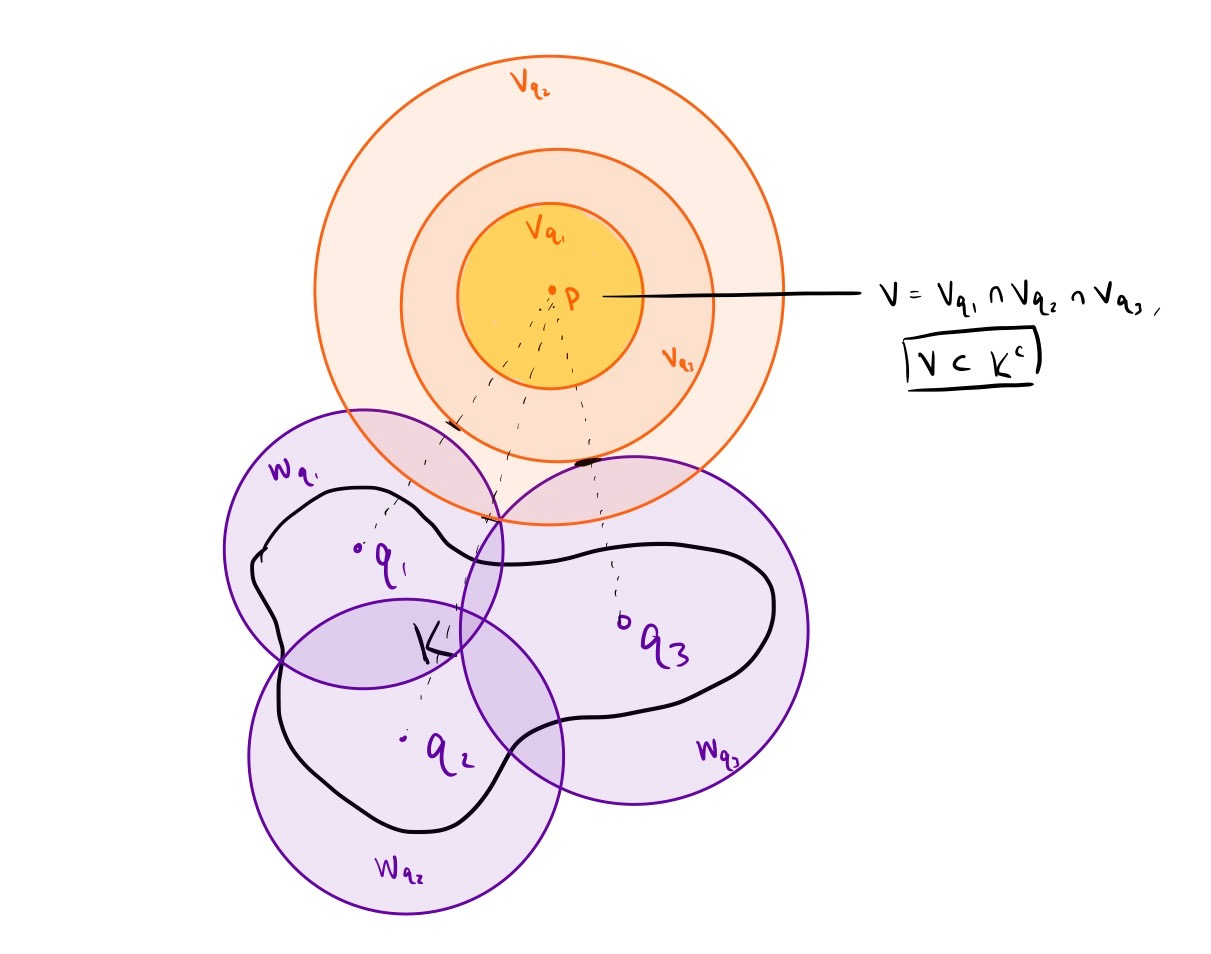
\includegraphics[width=10cm]{ClosedCompact.jpeg}
    \caption{Compact sets are closed.}
    \label{fig:galaxy}
\end{figure}
\begin{theorem}
    Closed subsets of compact sets are compact.
\end{theorem}
\begin{remark}
    Let $E$ be a closed subset of a compact space $K$. Note: $K$ being closed is a necessary condition! Let $\{V_{\alpha}\}$ be an open cover of $F$. Since $F^{c}$ is open, it follows that $\{V_{\alpha}\}\cup F^{c}$ is an open cover of $K$. Since $K$ is compact, we can obtain a finite subcover $\bigcup_{j=1}^{n}V_{i_{j}}\cup F^{c}$ of $K$. Since every element of $F$ is obviously not in $F^{c}$, it follows that $\bigcup_{j=1}^{n}V_{i_{j}}$ is an open cover of $F$.
\end{remark}
\begin{corollary}
    If $F$ is closed and $K$ compact, then $F\cap K$ is compact.
\end{corollary}
We will now begin to build machinery that is not only useful in its right, but also works to formulate a very important result of this chapter.
\begin{theorem}[Finite Intersection Theorem]
    If $\{K_{\alpha}\}$ is a collection of compact subsets of a metric space $X$ such that any intersection of finitely many elements of $\{K_{\alpha}\}$ is nonempty, then the arbitrary intersection $\bigcap_{\alpha}K_{\alpha}$ is also nonempty.
\end{theorem}
\begin{remark}
    To prove, fix a member $K_{1}$ of $K_{\alpha}$ and for each $K_{\alpha}$, let $G_{\alpha}=K_{\alpha}^{c}$. Assume, for sake of contradiction, that no single point of $K_{1}$ belongs to every $K_{\alpha}$. Then the collection $\{G_{\alpha}\}$ forms an open cover of the compact set $K_{1}$, so we can find a finite subcover $\{G_{\alpha_{i}}\}_{i=1}^{n}$ of $K_{1}$. But this means \[K_{1}\cap K_{\alpha_{1}}\cap\dotsi\cap K_{\alpha_{n}}\]is empty, a contradiction!
\end{remark}
\begin{corollary}[Nested Intersection Theorem]
    If $\{K_{n}\}$ is a sequence of nonempty compact sets such that $K_{n}\supset K_{n+1}$ for $n=1,2,\dotsc$, then $\bigcap_{i=1}^{\infty}K_{i}$ is nonempty.
\end{corollary}
\begin{theorem}
    Every infinite subset of a compact set $K$ has a limit point in $K$.
\end{theorem}
\begin{remark}
    To prove, suppose that $E\subset K$ does not have any limit points in itself. Then every point in $E$ has a neighborhood with exactly one element in $E$. The collection of those neighborhoods is an open cover for $E$, but obviously does not have a finite subcover.
\end{remark}
\begin{theorem}[Lemmas for Heine-Borel]
\listhack 
\begin{enumerate}
    \ii If $\{I_{n}\}$ is a sequence of (closed) intervals in $\RR$ such that $I_{n}\supset i_{n+1}$ for $n=1,2,\dotsc$, then $\bigcap_{n=1}^{\infty}I_{n}$ is not empty.
    \ii Let $k\in\NN$. If $\{I_{n}\}$ is a sequence of $k$-cells such that $I_{n}\supset i_{n+1}$ for $n=1,2,\dotsc$, then $\bigcap_{n=1}^{\infty}I_{n}\neq\emptyset$.
    \ii Every $k$-cell is compact.
\end{enumerate}
\end{theorem}
\begin{theorem}[Heine-Borel Theorem]
     Let $E$ in $\RR^{k}$. Then the following are equivalent:
     \begin{enumerate}
        \ii $E$ is closed and bounded.
        \ii $E$ is compact.
        \ii Every infinite subset of $E$ has a limit point in $E$.
     \end{enumerate}
\end{theorem}
\begin{remark}It should be noted that (2) and (3) are equivalent in \textit{every} metric space, but (1) does not, in general, imply (2) and (3).
\end{remark}
\begin{theorem}[Weierstrass]
    Every bounded infinite subset of $\RR^{k}$ has a limit point in $\RR^{k}$.
\end{theorem}
\begin{remark}
    If $E$ is a bounded infinite subset of $\RR^{k}$, then it is an infinite subset of a $k$-cell, which is compact. Thus $E$ has a limit point in that $k$-cell.
\end{remark}
\subsection{Perfect Sets}
\begin{theorem}
    Every nonempty perfect set in $\RR^{k}$ is uncountable.
\end{theorem}
\begin{remark}
    The perfect set $P$ has limit points, and is thus infinite. If $P$ were to be countable, we can enumerate the points $x_{1},x_{2},\dotsc$ and inductively construct the following sequence of neighborhoods $\{V_{n}\}$:
    \begin{enumerate}
        \ii $V_{1}$ is any neighborhood of $x_{1}$.
        \ii Suppose $V_{n}$ was constructed so that $V_{n}\cap P\neq\emptyset$. Every point of $P$ is a limit point, so there exists a neighborhood $V_{n+1}$ such that
        \begin{enumerate}
            \ii $\overline{V_{n+1}}\subset V_{n}$,
            \ii $x_{n}\not\in \overline{V_{n}}$,
            \ii $V_{n+1}\cap P\neq\emptyset$.
        \end{enumerate}
        \ii We can continue with our construction, as (c) satisfies the induction hypothesis.
    \end{enumerate}
    Let $K_{n}=\overline{V_{n}}\cap P$. $\overline{V_{n}}$ is closed and bounded, thus compact. By our construction, $x_{n}\not\in \overline{V_{n+1}}$, so there does not exist a point $p\in K$ such that $p\in \bigcap_{n=1}^{\infty}K_{n}$. But $K_{n}\subset P$, so the intersection $\bigcap_{n=1}^{\infty}$ is empty. But each $K_{n}$ is nonempty by (c) and $K_{n}\supset K_{n+1}$ by (a), so we have a contradiction with Corollary 2.57.
\end{remark}
\begin{corollary}
    Every open and closed interval in $\RR$ is uncountable. In particular, the set of all real numbers is uncountable.
\end{corollary}
\begin{example}[The Cantor Set]
    We will construct a perfect set in $\RR$ that does not contain any open intervals:
    \begin{enumerate}
        \ii Let $E_{0}=[0,1]$ and remove the segment $(\frac{1}{3},\frac{2}{3})$. Then let \[E_{1}=\left[0,\frac{1}{3}\right]\cup\left[\frac{2}{3},1\right].\]
        \ii Remove the middle thirds of these intervals, and let $E_{2}$ be the union 
        \[\left[0,\frac{1}{9}\right]\cup\left[\frac{2}{9},\frac{3}{9}\right]\cup\left[\frac{6}{9},\frac{7}{9}\right]\cup\left[\frac{8}{9},1\right].\]
        \ii We continue this construction to obtain a sequence of compact sets $E_{n}$ such that 
        \begin{enumerate}
            \ii $E_{1}\supset E_{2}\supset E_{3}\supset \dotsi$
            \ii $E_{n}$ is the union of $2^{-n}$ intervals, each of length $3^{-n}$.
        \end{enumerate}
    \end{enumerate}
    The set $P=\bigcup_{n=1}^{\infty}E_{n}$ is called the \vocab{Cantor Set}; $P$ is clearly compact, and nonempty by the Finite Intersection Theorem.
    \begin{itemize}
    \ii Notice that 
    \[\left(\frac{3k+1}{3^{m}},\frac{3k+2}{3^{m}}\right)\cap P=\emptyset,\]where $k,m\in\NN$. Notice that every open interval $(\alpha,\beta)$ contains a segment of the form $\left(\frac{3k+1}{3^{m}},\frac{3k+2}{3^{m}}\right)$ with $3^{-m}<\frac{\beta-\alpha}{6}$, so $P$ does not contain any open intervals.

    \ii To show $P$ is perfect, let $x\in P$, $S$ be any neighborhood of $X$ and $I_{n}$ the interval of $E_{n}$ containing $x$. We can choose $n$ large enough that $I_{n}\subset S$ (remember that $I_{n}$ gets smaller as $n$ increases), and let $x_{n}$ be the endpoint of $I_{n}$ such that $x\neq x_{n}$. We know from the construction of $P$ that $x_{n}\in P$, and thus $x$ is a limit point of $P$! 
    \end{itemize}
    An interesting property of the Cantor set is that it is an example of an uncountable set that has \textit{measure zero}.
\end{example}
\subsection{Connected Sets}
\begin{definition}
    Two subsets $A,B$ of a metric space $X$ are \vocab{separated} if both \[A\cap \overline{B}=\emptyset\quad\textrm{ and }\quad\overline{A}\cap B=\emptyset.\]A set $E\subset X$ is \vocab{connected} if $E$ is \textit{not} a union of two nonempty separated sets. 
\end{definition}    
\begin{remark}
    Obviously, separated sets are disjoint, but not every pair of disjoint set is separated! An illustrative example is as follows: $[0,1]$ and $(1,2)$ are \textit{not} separated since $1$ is a limit point of $(1,2)$, but $(0,1)$ and $(1,2)$ \textit{are} separated.
\end{remark}
\begin{theorem}
    A subset $E$ of $\RR$ is connected if, and only if, for any $x,y\in E$ with $x<z<y$, it must follow that $z\in E$.
\end{theorem}
\newpage



\section{Sequences and Series}
\prototype{Alternative harmonic series. What about it?}
\subsection{Convergent Sequences}
\begin{definition}
    A sequence $\{p_{n}\}$ in a metric space $X$ is said to \vocab{converge} to a point $p$ if for every $\epsilon>0$, there exists a $N\in\NN$ such that $d(p_{n},p)<\epsilon$ for all $n\geq N$.

    In this case, we also say $p$ is the limit of $\{p_{n}\}$, $p_{n}\rightarrow p$, or $\lim_{n\rightarrow\infty}p_{n}=p$. 

    If $\{p_{n}\}$ does not converge, it is said to \vocab{diverge}.
\end{definition}
\begin{remark}
    The notion of convergence is dependent on the embedding space of the sequence. For example, $\{1/n\mid n\in\NN\}$ converges in $\RR$ but not $(0,\infty)$.
\end{remark}
The set of all point $\{p_{n}\}$ is called the \emph{range} of $\{p_{n }\}$. If the range is bounded, was say the sequence itself is \textit{bounded}.

\begin{example}
\listhack 
\begin{enumerate}
    \ii If $s_{n}=1/n$, then $\lim_{n\rightarrow\infty}s_{n}=0$. The range is infinite, and the sequence is bounded.
    \ii If $s_{n}=n^{2}$, then the sequence $\{s_{n}\}$ is unbounded, is divergent, and has infinite range.
    \ii If $s_{n}=1+\frac{(-1)^{n}}{n}$, the sequence converges to 1, is bounded, and has infinite range.
    \ii If $s_{n}=i^{n}$, the sequence $\{s_{n}\}$ is divergent, is bounded, and has finite range.
    \ii If $s_{n}=1$, then $\{s_{n}\}$ converges to 1, is bounded, and has finite range.
\end{enumerate}
\end{example}
\begin{theorem} 
    Let $\{p_{n}\}$ be a sequence in a metric space $X$.
    \begin{enumerate}
        \ii \textbf{Tail phenomenon}: $\{p_{n}\}$ converges to $p\in X$ if, and only if, every neighborhood of $p$ contains $p_{n}$ for all but finitely many $n$.
        \ii \textbf{Uniqueness of limits}: If $p,p'\in X$, and if $\{p_{n}\}$ converges to $p$ and $p'$, then $p'=p$.
        \ii \textbf{Convergent sequences are bounded}: If $\{p_{n}\}$ converges, then $\{p_{n}\}$ is bounded.
        \ii \textbf{Limit points are the limit of a sequence}: If $E\subset X$ and if $p$ is a limit point of $E$, then there is a sequence $\{p_{n}\}$ in $E$ such that $p=\lim_{n\rightarrow\infty}p_{n}$.
    \end{enumerate}
\end{theorem}
\begin{remark}
    The proofs proceed as follows:
    \begin{enumerate}
        \ii If $p_{n}\rightarrow p$, then a neighborhood around $p$ of radius $r$ contains all but at most $N$ elements of $\{p_{n}\}$. Assuming the converse, then given some $\epsilon>0$, we know the neighborhood of radius $\epsilon$ contains all but finitely many $n$ elements of $p_{n}$, so we choose $N\geq n$.
        \ii For all $\epsilon>0$, there exists $N_{1},N_{2}\in\NN$ such that $d(p_{n},p_{1})<\frac{\epsilon}{2}$ and $d(p_{n},p_{2})<\frac{\epsilon}{2}$. So 
            \[d(p_{1},p_{2})\leq d(p_{1},p_{n})+d(p_{n},p_{2}) < \frac{\epsilon}{2}+\frac{\epsilon}{2}=\epsilon.\]
        \ii We know that there exists $N\in\NN$ such that $d(p_{n},p)<1$ for all $n\geq N$. Letting $r=\max\{1,d(p_{1},p),\dotsc,d(p_{N},p)\}$, we have that $d(p_{n},p)<r$ for all $n\in\NN$.
        \ii For every $n\in\NN$, there is a point $p_{n}\in E$  such that $d(p_{n},p)<\frac{1}{n}$. Given $\epsilon>0$, choose $N$ such that $N>\frac{1}{\epsilon}$. If $n>N$, then $d(p_{n},p)<\epsilon$.  \textbf{Note}: this technique of choosing $p_{n}$ such that $d(p_{n},p)<\frac{1}{n}$ is very useful.
    \end{enumerate}
\end{remark}
\begin{theorem}
    Suppose $\{s_{n}\},\{t_{n}\}$ are complex sequences, and $\lim_{n\rightarrow}s_{n}=s,\lim_{n\rightarrow\infty}t_{n}=t$. Then
    \begin{enumerate}
        \ii $\lim_{n\rightarrow\infty}(s_{n}+t_{n})=s+t$;
        \ii $\lim_{n\rightarrow\infty}cs_{n}=cs,$ $\lim_{n\rightarrow\infty}(c+s_{n})=c+s_{n}$, for any number $c$.
        \ii $\lim_{n\rightarrow\infty}s_{n}t_{n}=st$;
        \ii $\lim_{n\rightarrow\infty}\frac{1}{s_{n}}=\frac{1}{s}$, provided $s\neq 0$.
    \end{enumerate}
\end{theorem}
\begin{theorem}
    \listhack 
    \begin{enumerate}
        \ii Suppose $\vec{x_{n}}\in\RR^{k}$ and $\vec{x_{n}}=(\alpha_{1,n},\dotsc,\alpha_{k,n}).$ Then $\{\vec{x_{n}}\}$ converges to $\vec{x}=(\alpha_{1},\dotsc,\alpha_{k})$ if, and only if \[\lim_{n\rightarrow\infty}\alpha_{j,n}=\alpha_{j}\quad(1\leq j\leq k).\]
        \ii Suppose $\{\vec{x_{n}}\},\{\vec{y_{n}}\}$ are sequences in $\RR^{k}$, $\{\beta_{n}\}$ is a sequence of real numbers, and $\vec{x_{n}}\rightarrow\vec{x}$, $\vec{y_{n}}\rightarrow\vec{y_{n}}$, and $\beta_{n}\rightarrow\beta$. Then 
        \[\lim_{n\rightarrow\infty}(\vec{x_{n}}+\vec{y_{n}})=\vec{x}+\vec{y},\quad\lim_{n\rightarrow\infty}\vec{x_{n}}\cdot\vec{y_{n}}=\vec{x}\cdot\vec{y},\quad\lim_{n\rightarrow\infty}\beta_{n}\vec{x_{n}}=\beta\vec{x}.\]
    \end{enumerate}
\end{theorem}   
\begin{remark}
    The forward direction of (1) follows directly from the definition of the norm. Proving the converse, for each $\epsilon>0$ there exists a $N\in\NN$ such that if $n\geq N,$ then \[|\alpha_{j,n}-\alpha_{j}|<\frac{\epsilon}{\sqrt{k}}\]for $(1\leq j\leq k)$. Thus $n\geq N$ implies \[|\vec{x_{n}}-\vec{x}|=\left\{\sum_{j=1}^{k}|\alpha_{j,n}-\alpha_{j}|^{2}\right\}^{1/2}<\epsilon.\]
    (2) follows immediately from (1) and Theorem 3.6.
\end{remark}
\subsection{Subsequences}
\begin{definition}
    Given a sequence $\{p_{n}\}$, consider the increasing sequence $\{n_{k}\}$ of positive integers. The sequence $\{p_{n_{k}}\}$ is called a \vocab{subsequence} of $\{p_{n}\}$. If $\{p_{n_{k}}\}$ converges, its limit is called a \textit{subsequential limit} of $\{p_{n}\}$.
\end{definition}
\begin{remark}
    Obviously, $\{p_{n}\}$ converges to $p$ if, and only if, every subsequence of $\{p_{n}\}$ converges to $p$. Note that $\{p_{n}\}$ is a subsequence of itself.
\end{remark}
\begin{theorem}[Subsequences and Compactness]
    \listhack 
    \begin{enumerate}
        \ii A sequence in a compact metric space $X$ has a subsequence that converges to a point in $X$.
        \ii Every bounded sequence in $\RR^{k}$ has a convergent subsequence.
    \end{enumerate}
\end{theorem}
\begin{remark}
    The proof of (1) is trivial when the range of $\{p_{n}\}$ is finite. Otherwise, the range of $\{p_{n}\}$ is an infinite subset of a compact set, and thus has a limit point $p$. Since every neighborhood of $p$ contains infinitely many points in the range of $\{p_{n}\}$, we can choose $n_{1}\in\NN$ such that $d(p_{n_{1}},p)<1$, and $n_{i}>n_{i-1}$ such that $d(p_{n_{i}},p)<\frac{1}{i}$. (This argument should look familiar!) Moreover, (2) follows immediately from (1).
\end{remark}
\begin{theorem}
    The subsequential limits of a sequence $\{p_{n}\}$ in a metric space $X$ form a closed subset of $X$.
\end{theorem}
\begin{remark}
    The proof of this theorem involves showing that a limit point $q$ of $E^{*}$, the set of all subsequential limits of a sequence $\{p_{n}\}$, is contained in $E^{*}$. We first start by choosing some $n_{1}\in\NN$ such that $p_{n_{1}}\neq q$, and let $\delta=d(q,p_{n_{1}})$. If we can't find one, we're done. Assume inductively that $n_{1},\dotsc,n_{i-1}$ are already chosen. Because $q$ is a limit point of $E^{*}$, there exists some $x\in E^{*}$ such that $d(x,q)<2^{-i}\delta$. Since $x$ is a subsequential limit of $\{p_{n}\}$, there exists an $n_{i}>n_{i-1}$ such that $d(x,p_{n_{i}})< 2^{-i}\delta$. Then \[d(q,p_{n_{i}})\leq d(q,x)+d(x,p_{n_{i}})<(2^{-i}+2^{-i})\delta\]for $i\in\NN$. (This argument should look \textit{really} familiar!)
\end{remark}
\subsection{Cauchy Sequences}
\begin{definition}
    A sequence $\{p_{n}\}$ in a metric space $X$ is \vocab{Cauchy} if for every $\epsilon>0$, there exists a $N\in\NN$ such that $d(p_{n},p_{m})<\epsilon$ for all $n,m\geq N$.
\end{definition}
\begin{example}
    \listhack 
    \ii $\{\frac{1}{n}\mid n\in\NN\}$ is Cauchy. It is convergent in $\RR$ but \textit{not} convergent in $(0,\infty)$.
    \ii $\{3, 3.1, 3.14, 3.141, 3.1415, 3.14159,\dotsc\}$, where each successive term has one more digit of $\pi$ is Cauchy. It is convergent in $\RR$ but \textit{not} convergent in $\QQ$.
\end{example}
\begin{definition}
    Let $E$ be a nonempty subset of a metric space $X$, and let \[S=\{d(p,q)\mid p,q\in E\}.\]The supremum of $S$ is called the \vocab{diameter} of $E$.
\end{definition}
\begin{remark}
    If $\{p_{n}\}$ is a sequence in $X$ and $E=\{p_{N},p_{N+1},\dotsc\}$, then it's clear that $\{p_{n}\}$ is a Cauchy sequence if, and only if, $\lim_{N\rightarrow\infty}\textrm{diam }E_{N}=0.$
\end{remark}
\begin{theorem}
    \listhack 
    \begin{enumerate}
        \ii diam $\overline{E}=$ diam $E$.
        \ii If $\{K_{n}\}$ is a sequence of compact sets such that $K_{n}\supset K_{n+1}$ for all $n\in\NN$, and if \[\lim_{n\rightarrow\infty}\textrm{diam }K_{n}=0,\]then $\bigcap_{n=1}^{\infty}K_{n}$ consists of exactly one point.
    \end{enumerate}    
\end{theorem}
\begin{remark}
    Proving (1) consists of showing diam $E\leq$ diam $\overline{E}$ and diam $\overline{E}\leq$ diam $E$. Proving (2) is immediate from the Finite Intersection Theorem and a quick contradiction when assuming that the intersection has more than one point. 
\end{remark}
This machinery allows us to formalize an important intuition about Cauchy and convergent sequences: a limit is explicitly involved in the latter, but not the former.
\begin{theorem}
    \listhack 
    \begin{enumerate}
        \ii Every convergent sequence is Cauchy.
        \ii Every Cauchy sequence converges in a \textit{compact} metric space.
        \ii In $\RR^{k}$, every Cauchy sequence converges.
    \end{enumerate}
\end{theorem}
\begin{definition}
    A metric space is said to be \vocab{complete} if every Cauchy sequence in it converges.
\end{definition}
\begin{example}
    \listhack 
    \begin{enumerate}
        \ii All compact and Euclidean metric spaces are complete. 
        \ii Every closed subset of a complete metric space is complete.
        \ii $\QQ$ is not complete with $d(x,y)=|x-y|$.
    \end{enumerate}
\end{example}
\begin{definition}
    A sequence $\{s_{n}\}$ of real numbers is said to be
    \begin{enumerate}
        \item \vocab{monotonically increasing} if $s_{n}\leq s_{n+1}$ for $n\in\NN$;
        \item \vocab{monotonically decreasing} if $s_{n}\geq s_{n+1}$ for $n\in\NN$.
    \end{enumerate}
\end{definition}
\begin{theorem}[Monotone Convergence Theorem]
    A monotonic sequence converges if, and only if, it is bounded.
\end{theorem}
\begin{remark}
    Most of the proof is immediate. Suppose $s_{n}\leq s_{n+1}$ and $\{s_{n}\}$ is bounded. Then we can let $s$ be the least upper bound of $\{s_{n}\}$. Because $s=\sup\{s_{n}\}$, for each $\epsilon>0$ there exists an $N\in\NN$ such that \[s-\epsilon<s_{N}\leq s.\](Otherwise, $s-\epsilon$ would be an upper bound.) Then for all $n\geq N$, we have that $s-\epsilon<s_{n}\leq s$.
\end{remark}
\subsection{Upper and Lower Limits}
\begin{definition}
    If $\{s_{n}\}$ is a sequence of real numbers such that for every $M\in\RR$, there exists an $N\in\NN$ such that $n\geq N$ implies $s_{n}\geq M$, then we write \[s_{n}\rightarrow+\infty.\]
\end{definition}
A similar definition applies for limits to $-\infty$.
\begin{definition}
    Let $\{s_{n}\}\in \RR$ and $E=\{x\in\RR \mid s_{n_{k}}\rightarrow x\}$. The set $E$ contains all subsequential limits and possibly $+\infty,-\infty$. The \vocab{upper} and \vocab{lower limits} of $\{s_{n}\}$ are defined as follows:
    \[\limsup_{n\rightarrow\infty}s_{n}=\sup{E},\quad\quad\liminf_{n\rightarrow\infty}s_{n}=\inf{E}.\]
\end{definition}
\begin{theorem}
    Let $\{s_{n}\}$ be a sequence of real numbers and $E$ be defined as above. Then $\limsup{s_{n}}$ has the following two properties:
    \begin{enumerate}
        \ii $\limsup{s_{n}}\in E$,
        \ii If $x>\limsup{s_{n}}$, there is an $N\in\NN$ such that $n\geq N$ implies $s_{n}<x$.
    \end{enumerate}
    Of course, $\liminf$ has similar properties.
\end{theorem}
\begin{example}
    \listhack
    \begin{enumerate}
        \ii Let $\{s_{n}\}$ be a sequence of all the rationals (we can obtain such a sequence because $\QQ$ is countable). Then every real number is a subsequential limit and $\limsup_{n\rightarrow\infty}s_{n}=+\infty$, $\liminf_{n\rightarrow\infty}s_{n}=-\infty$.
        \ii Let $s_{n}=\frac{(-1)^{n}}{1+1/n}$. Then $\limsup_{n\rightarrow\infty}s_{n}=1$, and $\liminf_{n\rightarrow\infty}s_{n}=-1$.
        \ii For $\{s_{n}\}\in\RR$, it's the case that $\lim_{n\rightarrow\infty} s_{n}=s$ if, and only if \[\limsup_{n\rightarrow\infty}s_{n}=\liminf_{n\rightarrow\infty}s_{n}=s.\]
    \end{enumerate}
\end{example}
\begin{theorem}
    If $s_{n}\leq t_{n}$ for $n\geq N$, where $N$ is fixed, then \begin{align*}
        \liminf_{n\rightarrow\infty}s_{n} & \leq \liminf_{n\rightarrow\infty}t_{n},\\
        \limsup_{n\rightarrow\infty}s_{n} & \leq \limsup_{n\rightarrow\infty}t_{n}
    \end{align*}
\end{theorem}
\begin{example}
    \listhack 
    \ii If $p>0$, then $\lim_{n\rightarrow\infty}\frac{1}{n^{p}}=0$.
    \ii If $p>0$, then $\lim_{n\rightarrow\infty}\sqrt[n]{p}=1$.
    \ii $\lim_{n\rightarrow\infty}\sqrt[n]{n}=1$.
    \ii If $p>0$ and $\alpha\in\RR$, then $\lim_{n\rightarrow\infty}\frac{n^{\alpha}}{(1+p)^{n}}=0$.
    \ii If $|x|<1$, then $\lim_{n\rightarrow\infty}x^{n}=0$.
\end{example}
\subsection{Series}
\begin{definition}
    Given a sequence $\{a_{n}\}$, the infinite sum $\{a_{1}+a_{2}+\dotsi=\sum_{n=1}^{\infty}a_{n}$ is an \vocab{infinite series} or \textit{series}. The numbers $s_{n}=\sum_{k=1}^{n}a_{k}$ are the \vocab{partial sums} of the series, and if $\{s_{n}\}$ converges to $s$, then the series \emph{converges} and write \[\sum_{n=1}^{\infty}a_{n}=s.\]If $\{s_{n}\}$ diverges, the series is said to diverge.
\end{definition}
The Cauchy Criterion can be restated in the following form:
\begin{theorem}
    $\sum a_{n}$ converges if, and only if, for every $\epsilon>0$, there exists a $N\in\NN$ such that \[\left|\sum_{k=n}^{m}a_{k}\right|\leq \epsilon\]if $m\geq n\geq N.$
\end{theorem}
In other words:
\begin{theorem}[The Trivial Test]
    If $\sum a_{n}$ converges, then $\lim_{n\rightarrow\infty}a_{n}=0.$
\end{theorem}
\begin{remark}
    However, $a_{n}\rightarrow0$ is not a sufficient condition for convergence of $\sum a_{n}$. For example, the series $\sum_{n=1}^{\infty}\frac{1}{n}$ diverges.
\end{remark}
\begin{theorem}[Comparison Test]
    \listhack 
    \begin{enumerate}
        \item If $|a_{n}|\leq c_{n}$ for $n\geq N_{0}$, where $N_{0}\in\NN$, and if $\sum c_{n}$ converges, then $\sum a_{n}$ converges.
        \item If $a_{n}\geq d_{n}\geq 0$ for $n\geq N_{0}$, and if $\sum d_{n}$ diverges, then $\sum a_{n}$ alos diverges.
    \end{enumerate}
\end{theorem}
\subsection{Series of Non-negative Terms}
\begin{theorem}[Geometric Series]
    If $0\leq x<1$, then \[\sum_{n=0}^{\infty}x^{n}=\frac{1}{1-x}.\]If $x\geq 1$, the series diverges.
\end{theorem}
\begin{theorem}[Condensation Test]
    Suppose $a_{1}\geq a_{2}\geq \dotsi \geq 0$. Then the series $\sum_{n=1}^{\infty}a_{n}$ converges if, and only if, the series \[\sum_{k=0}^{\infty}2^{k}a_{2^{k}}=a_{1}+2a_{2}+4a_{4}+\dotsi\]converges.
\end{theorem}
\begin{theorem}[$p$-series]
    $\sum\frac{1}{n^{p}}$ converges if $p>1$ and diverges if $p\leq 1$.
\end{theorem}
\begin{theorem}
    If $p>1$, \[\sum_{n=2}^{\infty}\frac{1}{n(\log{n})^{p}}\]converges; if $p\leq 1$, the series diverges.
\end{theorem}
\subsection{The Number $e$}
\begin{definition}
    The number\[e=\sum_{n=0}^{\infty}\frac{1}{n!}.\]
\end{definition}
\begin{theorem}
    \[\lim_{n\rightarrow\infty}\left(1+\frac{1}{n}\right)^{n}=e.\]
\end{theorem}
\begin{theorem}
    $e$ is irrational. 
\end{theorem}

\subsection{The Root and Ratio Tests}
\begin{theorem}[Root Test]
    Given $\sum a_{n}$, put $\alpha=\limsup_{n\rightarrow\infty}\sqrt[n]{|a_{n}|}.$ Then 
    \begin{enumerate}
        \item If $\alpha<1$, $\sum a_{n}$ converges;
        \item $\alpha>1$, $\sum a_{n}$ diverges;
        \item If $\alpha=1$, the test is inconclusive.
    \end{enumerate}
\end{theorem}
\begin{theorem}[Ratio Test]
    The series $\sum a_{n}$
    \begin{enumerate}
        \item converges if $\limsup_{n\rightarrow\infty}\left|\frac{a_{n+1}}{a_{n}}\right|<1$,
    \item diverges if $\left|\frac{a_{n+1}}{a_{n}}\right|\geq 1$ for all $n\geq n_{0}$, where $n_{0}$ is a fixed integer.
        \item If $\lim a_{n+1}/a_{n}=1$, the test is inconclusive.
    \end{enumerate}
\end{theorem}
\begin{example}
    \listhack 
    \ii The series $\frac{1}{2}+\frac{1}{3}+\frac{1}{2^{2}}+\frac{1}{3^{2}}+\frac{2^{3}}+\frac{3^{3}}+\dotsi$ is shown to be convergent by the root test, but the ratio test is inconclusive.
    \ii The same is true for the series $\frac{1}{2}+1+\frac{1}{8}+\frac{1}{4}+\frac{1}{32}+\frac{1}{16}+\dotsi$.
\end{example}
\begin{remark}
    The ratio test is usually easier to apply than the root test, but the root test has wider \textit{scope}. In other words, whenever the ratio test shows convergence, the root test does too. Whenever the root test is inconclusive, the ratio test is too.
\end{remark}
\begin{theorem}
    For any sequence $\{c_{n}\}$ of positive numbers:
    \begin{enumerate}
        \item $\liminf_{n\rightarrow\infty}\frac{c_{n+1}}{c_{n}}\leq \liminf_{n\rightarrow\infty}\sqrt[n]{c_{n}},$
        \item $\limsup_{n\rightarrow\infty}\sqrt[n]{c_{n}}\leq \limsup_{n\rightarrow\infty}\frac{c_{n+1}}{c_{n}}.$
    \end{enumerate}
\end{theorem}

\subsection{Power Series}
\begin{definition}
    Given $\{c_{n}\}\in\CC$, the series \[\sum_{n=0}^{\infty}c_{n}z^{n}\]is called a \vocab{power series}, with \textit{coefficients} $c_{n}$. The series will converge or diverge based on $z$; every power series has an associated \textit{circle of convergence}, such that the power series will converge if $z$ is in the interior of the circle and diverge otherwise.
\end{definition}
\begin{theorem}
    Given the power series $\sum c_{n}z^{k}$, put \[\alpha=\limsup_{n\rightarrow\infty}\sqrt[n]{|c_{n}|},\quad R=\frac{1}{\alpha}.\](If $\alpha=0$, then $R=+\infty;$ if $\alpha=+\infty$, then $R=0$.) $\sum c_{n}z^{n}$ converges if $|z|<R$, and diverges if $|z|>R$. 
    
\end{theorem}
\begin{remark}
    The proof consists of applying the root test to $a_{n}=c_{n}z^{n}$:
    \[\limsup_{n\rightarrow\infty}\sqrt[n]{|a_{n}|}=|z|\limsup_{n\rightarrow\infty}\sqrt[n]{c_{n}}=\frac{|z|}{R}.\]

    Note that we can also use the ratio test to obtain a radius of convergence, but it might not capture all $z$ values for which the power series converges.
\end{remark}
\begin{example}
    \listhack 
    \begin{enumerate}
        \ii $\sum n^{n}z^{n}$ has $R=0$.
        \ii $\sum\frac{z^{n}}{n!}$ has $R=+\infty$. (It is easier to use the ratio test in this example).
        \ii $\sum \frac{z^{n}}{n}$ has $R=1$, and diverges if $z=1$ but converges for other $|z|=1$.
        \ii $\sum z^{n}$ has $R=1$. If $|z|=1$, the series diverges since the limit of $z_{n}$ is not 0.
        \ii $\sum\frac{z^{n}}{n^{2}}$ has $R=1$, and converges for all $z$ with $|z|=1$, by comparison with $1/n^{2}$.
    \end{enumerate}
\end{example}
\subsection{Summation By Parts}
\begin{theorem}
    Let $\{a_{n}\},\{b_{n}\}$ be sequences, and let $A_{n}=\sum_{k=0}^{n}a_{k}$ if $n\geq 0$; and let $A_{-1}=0$. Then if $0\leq p\leq q$, we have \[\sum_{n=p}^{q}a_{n}b_{n}=\sum_{n=p}^{q-1}A(b_{n}-b_{n+1})+A_{q}b_{q}-A_{p-1}b_{p}.\]
\end{theorem}
\begin{remark}
    Summation by parts is especially useful when investigating series of the form $\sum a_{n}b_{n}$, particularly when $\{b_{n}\}$ is monotonic.
\end{remark}
\begin{theorem}
    Suppose 
    \begin{enumerate}
        \item The partial sums $A_{n}$ of $\sum a_{n}$ form a bounded sequence;
        \item $b_{0}\geq b_{1}\geq b_{2}\geq \dotsi$;
        \item $\lim_{n\rightarrow\infty}b_{n}=0$.
    \end{enumerate}
    Then $\sum a_{n}b_{n}$ converges.
\end{theorem}
\begin{theorem}[Alternating Series Test]
    Suppose 
    \begin{enumerate}
        \item $|c_{1}|\geq |c_{2}|\geq |c_{3}|\geq \dotsi$;
        \item $c_{2m-1}\geq 0$, $c_{2m\leq 0}$, for $m\in\NN$.
        \item $\lim_{n\rightarrow\infty}c_{n}=0$.
    \end{enumerate}
    Then $\sum c_{n}$ converges.
\end{theorem}   
\begin{example}[Alternating Harmonic Series]
    Let $a_{n}=\frac{(-1)^{n}}{n}$. Then $\sum a_{n}$ converges.
\end{example}
\begin{theorem}
    Suppose the radius of convergence of $\sum c_{n}z^{n}$ is 1, and suppose $c_{0}\geq c_{1}\geq c_{2}\geq \dotsi$, and $\lim_{n\rightarrow\infty}c_{n}=0$. Then $\sum c_{n}z^{n}$ converges at every point on the circle $|z|=1$, except possibly at $z=1$.
\end{theorem}
\subsection{Absolute Convergence}
\begin{definition}
    A series $\sum a_{n}$ \vocab{converges absolutely} if the series $\sum|a_{n}|$ converges.
\end{definition}
\begin{remark}
    The comparison, root, and ratio tests are really tests for absolute convergence and cannot give any information about non-absolutely convergent series.
\end{remark}

\subsection{Addition and Multiplication of Series}
\begin{theorem}
    If $\sum a_{n}=A$ and $\sum b_{n}=B$, then $\sum (a_{n}+b_{n})=A+B$, and $\sum c a_{n}=cA$ for any fixed $c$.
\end{theorem}
\begin{definition}[Cauchy]
    Given $\sum a_{n}$ and $\sum b_{n}$, the \vocab{Cauchy product} of the two series is \[c_{n}=\sum_{k=0}^{n}a_{k}b_{n-k}\]
\end{definition}
\begin{remark}
    If $A_{n}=\sum_{k=0}^{n}a_{k}$, $B_{n}=\sum_{k=0}^{n}b_{k}$, $C_{n}=\sum_{k=0}^{n}c_{k}$, and $A_{n}\rightarrow A$, $B_{n}\rightarrow B$, and $C_{n}\rightarrow C$, it is not necessarily the case that $\{C_{n}\}$ converges to $AB$.
\end{remark}
\begin{example}
    The series \[\sum_{n=0}^{\infty}\frac{(-1)^{n}}{\sqrt{n+1}}=1-\frac{1}{\sqrt{2}}+\frac{1}{\sqrt{3}}-\frac{1}{\sqrt{4}}+\dotsi\]converges, but the Cauchy product of the series with itself does not converge.
\end{example}
\begin{theorem}
    Suppose 
    \begin{enumerate}
        \ii $\sum_{n=0}^{\infty}a_{n}$ converges absolutely,
        \ii $\sum_{n=0}^{\infty}a_{n}=A$,
        \ii $\sum_{n=0}^{\infty}b_{n}=B$,
        \ii $c=\sum_{k=0}^{n}a_{k}b_{n-k}$ for $n=0,1,\dotsc$.
    \end{enumerate}
    Then \[\sum_{n=0}^{\infty}c_{n}=AB\]
\end{theorem}
In other words, the product of two convergent series converges to the the product of their individual limits if at least one of the two series converges absolutely.

\begin{theorem}
    If the series $\sum a_{n}$, $\sum b_{n}$, and $c_{n}$ converge to $A, B, C$, and $c_{n}=a_{0}b_{n}+\dotsi+a_{n}b_{0}$, then $C=AB$.
\end{theorem}
Here, no assumptions are made about absolute convergence.
 
\subsection{Rearrangements}
\begin{definition}
    Let $\{k_{n}\}$ be a sequence in which every positive integer appears exactly once. Putting $a_{n}'=a_{k_{n}}$, we say that $\sum a_{n}'$ is a \vocab{rearrangement} of $\sum a_{n}$.
\end{definition}
\begin{example}
    Consider the convergent series 
    \[1-\frac{1}{2}+\frac{1}{3}-\frac{1}{4}+\dotsi\]and one of its rearrangements 
    \[1+\frac{1}{3}-\frac{1}{2}+\frac{1}{5}+\frac{1}{7}-\frac{1}{4}+\frac{1}{9}+\frac{1}{11}-\frac{1}{6}+\dotsi\]in which two positive terms are always followed by one negative. If $s$ is the first sum, then $s<1-\frac{1}{2}+\frac{1}{3}=\frac{5}{6}.$ Since $\frac{1}{4k-3}+\frac{1}{4k-1}-\frac{1}{2k}>0$ for $k\geq 1$, we see that $s_{3}'<s_{6}'<s_{9}'<\dotsi$ where $s_{n}'$ is $n$th partial sum of the second sum. Thus $\limsup_{n\rightarrow\infty}s_{n}'>s_{3}'=\frac{5}{6}$, so the two sums do not converge to the same value (if any).
\end{example}
\begin{theorem}
    Let $\sum a_{n}$ be a series of real numbers which converges, but not absolutely. Suppose \[-\infty\leq \alpha\leq \beta\leq \infty.\]Then there exists a rearrangement $\sum a_{n}'$ with partial sums $s_{n}'$ such that \[\liminf_{n\rightarrow\infty}s_{n}'=\alpha,\quad\quad \limsup_{n\rightarrow\infty}s_{n}'=\beta.\]
\end{theorem}
\begin{theorem}
    If $\sum a_{n}$ is a series of complex numbers which converge absolutely, then every rearrangement of $\sum a_{n}$ converges, and they all converge to the same sum.
\end{theorem}
\newpage


\section{Continuity}
\subsection{Limits of Functions}
\begin{definition}
    Let $X$ and $Y$ be metric spaces, $E\subset X$, $f:E\rightarrow Y$, and $p$ is a limit point of $E$. We write \[f(x)\rightarrow q\textrm{ as }x\rightarrow p,\quad\textrm{or}\quad\lim_{x\rightarrow p}f(x)=q\]if there is a point $q\in Y$ such that for every $\epsilon>0$, there exists a $\delta>0$ such that \[d_{Y}(f(x),q)<\epsilon\]for all points $x\in E$ for which \[0<d_{X}(x,p)<\delta.\]
\end{definition}
\begin{remark}
    A few notes:
    \begin{enumerate}
        \ii $X$ and $Y$ might have different distance functions, so we denote each as $d_{X}$ and $d_{Y}$ to prevent ambiguity.
        \ii It's of course necessary that $p\in X$, but $p$ does \textit{not} need to be in $E$. In fact, even \textit{if} $p\in E$, it might be the case that $\lim_{x\rightarrow p}f(x)\neq f(p)$.
    \end{enumerate}
\end{remark}    
\begin{theorem}
    Assume all variables from Definition 4.1 carry the same meaning. Then \[\lim_{x\rightarrow p}f(x)=q\]if, and only if, \[\lim_{n\rightarrow\infty}f(p_{n})=q\]for every sequence $\{p_{n}\}$ in $E$ such that $p_{n}\neq p$ and $\lim_{n\rightarrow\infty}p_{n}=p$.
\end{theorem}
\begin{remark}
    The proof is a simple exercise in symbolic manipulation. For the forward direction, choose a sequence $\{p_{n}\}$ that converges to $p$ (with $p_{n}\neq p$), and let $\epsilon>0$. Then there exists a $\delta>0$ such that $d(f(x),q)<\epsilon$ if $0<d(x,p)<\delta$. Furthermore, there exists an $N\in\NN$ such that $d(p_{n},p)<\delta$, and thus $d(f(p_{n}),q)<\epsilon$ for every $n\geq N$. 
    
    Conversely, we proceed by contraposition, supposing $\lim_{x\rightarrow p}f(x)\neq q$. Then there exists an $\epsilon>0$ such that for every $\delta>0$, there exists an $x\in X$ such that $d(f(x),q)\geq \epsilon$ if $0<d(x,p)<\delta$. We can now construct a sequence that converges to $p$ as follows:
    \begin{enumerate}
        \ii For $n\in\NN$, let $\delta_{n}=\frac{1}{n}$.
        \ii Pick $x_{n}$ such that $d(f(x_{n}),q)\geq\epsilon$ if $0<d(x_{n},p)<\delta_{n}$.
    \end{enumerate}
    The sequence $\{x_{n}\}$ converges to $p$ and $x_{n}\neq p$, but $\lim_{n\rightarrow\infty}f(x_{n})\neq q$.
\end{remark}
\begin{definition}[Sums and Products of Functions]
    For complex functions $f,g$ defined on $E$, we have that 
    \[(f+g)(x)=f(x)+g(x)\quad\textrm{and}\quad (fg)(x)=f(x)g(x)\]
    and if $f(x)\geq g(x)$ for every $x\in E$, we sometimes write $f\geq g$.
\end{definition}
\begin{theorem}
    Suppose $E\subset X$, $p$ is a limit point of $E$, $f,g$ are complex functions on $E$, and $\lim_{x\rightarrow p}f(x)=A, \lim_{x\rightarrow p}g(x)=B$. Then
    \begin{enumerate}
        \item $\lim_{x\rightarrow p}(f+g)(x)=A+B$;
        \item $\lim_{x\rightarrow p}(fg)(x)=AB$;
        \item $\lim_{x\rightarrow p}\left(\frac{f}{g}\right)(x)=\frac{A}{B}$ if $B\neq 0$.
    \end{enumerate}
\end{theorem}

\subsection{Continuous Functions}
\begin{definition}
    Suppose $X,Y$ are metric spaces, $E\subset X$, $p\in E$, and $f$ maps $E$ into $Y$. Then $f$ is said to be \vocab{continuous at $p$} if for every $\epsilon>0$, there exists a $\delta>0$ such that \[d_{Y}(f(x),f(p))<\epsilon\]for all points $x\in E$ for which $d_{X}(x,p)<\delta$.
\end{definition}
\begin{remark}
    \begin{itemize}
        \ii If $f$ is continuous at \textit{every} point of $E$, then $f$ is said to be \vocab{continuous on $E$}. 
        \ii Also of note is that $f$ must be defined at $p$ in order for it to be continuous at $p$. 
        \ii If $p$ is an isolated point of $E$, then every function with $E$ as its domain is (vacuously) continuous at $p$.
    \end{itemize}
\end{remark}

\begin{theorem}[Alternate Definition of Continuity at a Point]
    Assume that $p$ is a limit point of $E$. Then $f$ is continuous at $p$ if, and only if, \[\lim_{x\rightarrow p}f(x)=f(p).\]
\end{theorem}
\begin{theorem}[Composition of Functions]
    Suppose $X,Y,Z$ are metric spaces, $E\subset X$, $f:E\rightarrow Y$, $g:f(E)\rightarrow Z$, and $h$ is defined as
    \[h(x)=g(f(x))\quad(x\in E).\]If $f$ is continuous at a point $p\in E$ and if $g$ is continuous at the point $f(p)$, then $h$ is continuous at $p$.

    This function $h$ is called the \vocab{composition} or the \textit{composite} of $f$ and $g$. We frequently use the notation $h=g\circ f$.
\end{theorem}
\begin{remark}
    The proof is fairly straightforward from the definition of continuity at a point.
\end{remark}
\begin{theorem}[Continuity and Inverse Images]
    A mapping $f$ of a metric space $X$ into a metric space $Y$ is continuous on $X$ if, and only if, $f^{-1}(V)$ is open in $X$ for every open set $V$ in $Y$.
\end{theorem}
\begin{remark}
    This is oftentimes more useful than the first definition of continuity.

    To prove, let $f$ be continuous on $X$ and $V$ be an open set in $Y$. Let $y=f(p)\in V$, and since $V$ open, there exists some neighborhood $N_{\epsilon}(y)\subset V$. Since $f$ continuous, there exists a $\delta >0$ such that $d(f(x),f(p))<\epsilon$ if $d(x,p)<\delta$. Then $x\in f^{-1}(V)$ as soon as $d(x,p)<\delta$.

    Conversely, suppose $f^{-1}(V)$ is open in $X$ for an open set $V\in Y$. Choose some $p\in X$ and let $\epsilon>0$. Notice that $V=\{y\in Y\mid d(f(p),y)<\epsilon\}$ is an open set, so $f^{-1}(V)$ is also open. In other words, there exists a $\delta>0$ such that $x\in f^{-1}(x)$ (and thus $f(x)\in V$ or $d(f(x),f(p))<\epsilon$) if $d(x,p)<\delta$.
\end{remark}
\begin{corollary}
    A mapping $f$ of a metric space $X$ into a metric space $Y$ is continuous if, and only if, $f^{-1}(C)$ is closed in $X$ for every closed set $C$ in $Y$.
\end{corollary}
\begin{theorem}[Sums, Products, and Quotients of Continuous Functions are Continuous]
    Let $f,g$ be complex continuous functions on a metric space $X$. Then $f+g,fg,$ and $f/g$ are continuous on $X$. (Assuming of course that $g\neq 0$ in the last statement.)
\end{theorem}
\begin{theorem}
    \listhack 
    \begin{enumerate}
        \ii Let $f_{1},f_{2},\dotsc,f_{k}$ be real functions on a metric space $X$, and $\vec{f}$ be a mapping from $X$ into $\RR^{k}$ defined by 
        \[\vec{f}(x)=(f_{1}(x),\dotsc,f_{k}(x))\quad(x\in X);\]then $f$ is continuous if, and only if, each of the functions $f_{1},\dotsc,f_{k}$ is continuous.
        \ii If $\vec{f},\vec{g}$ are continuous mappings of $X$ into $\RR^{k}$, then $\vec{f}+\vec{g}$ and $\vec{f}\cdot \vec{g}$ are continuous on $X$.
    \end{enumerate}
\end{theorem}
\begin{remark}
    \ii The functions $f_{1},\dotsc,f_{k}$ are called the \vocab{components} of $f$.
\end{remark}
\begin{example}
    Every polynomial and rational function (given denominator zero, of course) is continuous on $\RR^{k}$.
\end{example}
\begin{remark}
    When referring to a function $f$, we lose nothing from discarding the complement of the domain of $f$, so we shall talk about continuous mappings of one metric space into another instead of mappings of subsets, and can do so without ambiguity.
\end{remark}
\subsection{Continuity and Compactness}
\begin{definition}
    A mapping $\vec{f}$ of a set $E$ into $\RR^{k}$ is said to be \vocab{bounded} if there exists $M\in\RR$ such that $|\vec{f}|\leq M$ for all $x\in E$.
\end{definition}
\begin{theorem}[Continuous Images of Compact Sets are Compact]
    Suppose $X$ is compact, and $f:X\rightarrow Y$ is continuous. Then $f(X)$ is compact.
\end{theorem}
\begin{remark}
    Note that $f(f^{-1}(E))\subset E$, where $E\subset Y$. (If $E\subset X$, then $f^{-1}(f(E))\supset E$.) To prove the above theorem, let $\{G_{\alpha}\}$ be an open cover of $f(X)$, use the continuity of $f$ to see that $\{f(G_{\alpha})\}$ is an open cover of $X$, and use the compactness of $X$ to obtain a finite subcover.
\end{remark}
We can observe some consequences of Theorem 4.21:
\begin{theorem}
    If $X$ is compact and $\vec{f}:X\rightarrow\RR^{k}$ is continuous, then $\vec{f}(X)$ is closed and bounded. Thus $\vec{f}$ is bounded.
\end{theorem}
\begin{theorem}[Extreme Value Theorem]
    Suppose $X$ is compact, $f:X\rightarrow\RR$, and $M=\sup_{p\in X}f(p)$, $m=\inf_{p\in X}f(p)$. Then there exist points $p,q\in X$ such that $f(p)=M$ and $f(q)=m$.
\end{theorem}
\begin{remark}
    This directly follows from the fact that a closed and bounded sets in $\RR$ contains its supremum and infimum.
\end{remark}
\begin{theorem}[Inverses of Continuous Bijections are Continuous]
    Suppose $f$ is a continuous 1-1 mapping of a compact metric space $X$ onto a metric space $Y$ (in other words, a bijection from $X$ to $Y$). Then the inverse mapping $f^{-1}$ defined on $Y$ by \[f^{-1}(f(x))=x\quad(x\in X)\]is a continuous mapping of $Y$ onto $X$.
\end{theorem}
\begin{remark}
    It suffices to show that $f(V)$ is open if $V\subset X$ is open. Notice that $f(V^{c})$ is compact, thus closed, and since $f$ is a bijection, we have $f(V^{c})=f(V)^{c}$ so $f(V)$ is open. 
\end{remark}
\begin{definition}
    Let $f:X\rightarrow Y$. We say $f$ is \vocab{uniformly continuous} on $X$ if for every $\epsilon>0$, there exists a $\delta>0$ such that \[d_{Y}(f(p),f(q))<\epsilon\]for all $p,q\in X$ for which $d_{X}(p,q)<\delta$.
\end{definition}
Notice there are subtle differences between uniform continuity and continuity:
\begin{itemize}
    \ii Continuity can be defined at a single point, whereas uniform continuity is inherently defined in terms of a set.
    \ii If $f$ is continuous on $X$, it is possible to find, for each $\epsilon>0$ and each point $p\in X$, a number $\delta>0$, which depends on both $p$ \textit{and} $\epsilon$. 
    \ii On the other hand, if $f$ is uniformly continuous on $X$, then it is possible for each $\epsilon>0$ to find \textit{one} number $\delta>0$ that will work for \textit{all} points $p$ of $X$.
    \ii It follows from the logic above that every uniformly continuous function is continuous (but the converse does not necessarily hold.)
\end{itemize}
\begin{theorem}
    Let $X$ be compact, and $f:X\rightarrow Y$ be continuous. Then $f$ is uniformly continuous on $X$.
\end{theorem}
\begin{remark}
    To prove, we have to show that for some $\epsilon>0$, there exists a $\delta>0$ such that $d(f(p),f(q))<\epsilon$ if $d(p,q)<\delta$.

    Let $\epsilon>0$, and for each $p\in X$, define $\phi(p)$ such that for $q\in X$, 
    \[d(p,q)<\phi(p)\Rightarrow d(f(p),f(q))<\frac{\epsilon}{2}.\]Now, let \[J(p)=\{q\in X\mid d(p,q)<\frac{1}{2}\phi(p).\}\]
    It should be clear that the collection $\{J_{p}\}$ is an open cover of the compact set $X$, so there exist a finite set of points $p_{1},\dotsc,p_{n}\in X$ such that \[X\subset J(p_{1})\cup\dotsi\cup J(p_{n}).\]We can choose $\delta=\frac{1}{2}\min[\phi(p_{1}),\dotsc,\phi(p_{n})]$, and because our list is finite, we know $\delta>0$. (Notice that this is not necessarily the case for an infinite list of points.) Now, let $p,q\in X$ such that $d(p,q)<\delta$. Then there exists some $m$, with $1\leq m\leq n$, such that $p\in J(p_{m}),$ so \[d(p,p_{m})<\frac{1}{2}\phi(p_{m}).\]Moreover, notice that \begin{align*}
        d(q,p_{m}) & \leq d(p,q)+d(p,p_{m})\\
        & <\delta+\frac{1}{2}\phi(p_{m})\\
        & \leq \phi(p_{m})
    \end{align*}
    Thus $d(f(p),f(p_{m}))<\frac{\epsilon}{2}$ and $d(f(q),f(p_{m}))<\frac{\epsilon}{2}$. So \[d(f(p),f(q))\leq d(f(p),f(p_{m}))+d(f(q),f(p_{m}))<\epsilon.\]
\end{remark}
\begin{theorem}
    Let $E$ be a non-compact set in $\RR$. Then 
    \begin{enumerate}
        \ii There exists an unbounded continuous function on $E$.
        \ii There exists a continuous and bounded function on $E$ with no maximum.
        \ii If $E$ is bounded, then there exists a continuous function on $E$ that is not uniformly continuous.
    \end{enumerate}
\end{theorem}
\begin{example}
    \listhack 
    \begin{enumerate}
        \ii If $E$ is bounded, and there exists a limit point $x_{0}$ of $E$ that is not a point of $E$, then \[f(x)=\frac{1}{x-x_{0}}\quad(x\in E)\]is continuous on $E$, but unbounded. In fact, if we let $\epsilon>0$, $\delta>0$, and choose a point $x\in E$  such that $|x-x_{0}|<\delta$, we can take $t$ close enough to $x_{0}$ so that we can make the difference $|f(t)-f(x)|>\epsilon$, despite $|t-x|<\delta$. Since $\delta$ is arbitrary, $f$ is not uniformly continuous on $E$.
        \ii The function \[g(x)=\frac{1}{1+(x-x_{0})^{2}}\quad(x\in E)\]is continuous on $E$ and bounded between $0$ and $1$. Clearly, $\sup_{x\in E}g(x)=1$, but $g(x)<1$ for all $x\in E$ so $g$ has no maximum on $E$.
        \ii Assume $E$ is unbounded. Then $f(x)=x$ is continuous but unbounded, $h(x)=\frac{x^{2}}{1+x^{2}}$ is continuous and bounded with no maximum ($\sup_{x\in E}h(x)=1$). 
        \ii If we omit boundedness as a condition from (3), then the statement would be false. For example, if $E=\ZZ$, then every function on $E$ would be uniformly continuous (take $\delta<1$).
    \end{enumerate}
\end{example}
We'll now illustrate with an example that compactness of the domain is also essential in ensuring the inverse mapping of a continuous bijection is continuous.
\begin{example}
    Let $X=[0,2\pi)\subset \RR$, $Y=\{\vec{y}\in\RR^{2}\mid |\vec{y}|=1\}$. Then define $\vec{f}:X\rightarrow{Y}$ as follows:
    \[\vec{f}(t)=(\cos{t},\sin{t})\quad(0\leq t<2\pi).\]We will take for granted that both cosine and sine are continuous and have nice enough periodic properties such that $\vec{f}$ is a bijection. 

    Notice that $f^{-1}$ is not continuous at $(1,0)=\vec{f}(0)$, with, of course, the culprit being that $X$ is not compact. (It might be intriguing to see that $Y$ \textit{is} compact!)
\end{example}
\subsection{Continuity and Connectedness}
\begin{theorem}[The Image of a Connected Set Under a Continuous Mapping is Connected]
    Let $f:X\rightarrow Y$ be continuous and $E\subset X$ be connected. Then $f(E)$ is connected.
\end{theorem}
\begin{remark}
    To prove, we will suppose to the contrary that $f(E)=A\cup B$, where $A,B$ are separated. Let \[G=E\cap f^{-1}(A),\quad H=E\cap f^{-1}(B).\]Then $E=G\cup H$, since $A,B$ separated. Notice $A\subset \overline{A},$ so $G\subset f^{-1}(\overline{A})$, and since $f^{-1}(\overline{A})$ is closed by the continuity of $f$, it follows that $\overline{G}\subset f^{-1}(\overline{A})$. Then $f(\overline{G})\subset \overline{A}$. Notice \[f(\overline{G})\cap f(H)\subset \overline{A}\cap B=\emptyset,\]so $\overline{G}\cap H=\emptyset$, and similarly, $G\cap \overline{H}=\emptyset$. Thus $G,H$ are separated, a clear contradiction!
\end{remark}
\begin{theorem}[Intermediate Value Theorem]
    Let $f$ be a continuous real function on the interval $[a,b]$. If $f(a)<f(b)$ and if $c$ is a number such that $f(a)<c<f(b)$, then there exists a point $x\in(a,b)$ such that $f(x)=c$.
\end{theorem}
\begin{remark}
    The converse might seem to be true (that if for any two points $x_{1}<x_{2}$ and for any $c\in(f(x_{1}),f(x_{2}))$, there exists an $x\in(x_{1},x_{2})$ such that $f(x)=c$, then $f$ is continuous), but consider the following:
    \[f(x)=\begin{cases}
        \sin(\frac{1}{x}) & (x\neq 0),\\
        0 & (x=0).
    \end{cases}\]
    We will show later that this function is not continuous.
\end{remark}

\subsection{Discontinuities}
If $x$ is a point in the domain of the function $f$ at which $f$ is not continuous, we say that $f$ is \vocab{discontinuous} at $x$.
\begin{definition}
    Let $f$ be defined on $(a,b)$. Consider any point $x$ such that $a\leq x < b$. We define the \textit{right-hand limit} of $f$ at $x$ as $f(x+)=q$ if $f(t_{n})\rightarrow q$ as $n\rightarrow\infty$, for all sequences $\{t_{n}\}$ in $(x,b)$ such that $t_{n}\rightarrow x$. To obtain the definition of the \textit{left-hand limit} $f(x-)$, for $a<x\leq b$, we restrict ourselves to sequences $\{t_{n}\}$ in $(a,x)$.
\end{definition}
\begin{remark}
    At any point $x\in (a,b)$, $\lim_{t\rightarrow x}f(t)$ exists if, and only if,\[f(x+)=f(x-)=\lim_{t\rightarrow x}f(t).\]
\end{remark}
\begin{definition}
    Let $f$ be defined on $(a,b)$. 
    \begin{enumerate}
        \ii If $f$ is discontinuous at $x$ and if $f(x+)$ and $f(x-)$ exist, then $f$ is said to have a discontinuity of the \textit{first kind}, or a \vocab{simple discontinuity} at $x$.
        \ii Otherwise, $f$ has a discontinuity of the \textit{second kind}.
    \end{enumerate}
\end{definition}
\begin{remark}
    There are two ways a function can have a simple discontinuity:
    \begin{enumerate}
        \ii $f(x+)\neq(x-)$,
        \ii $f(x+)=f(x-)\neq f(x)$.
    \end{enumerate}
\end{remark}
\begin{example}
    Define 
    \[f(x)=\begin{cases}
        1 & (x\in \QQ),\\
        0 & (x\not\in \QQ).
    \end{cases}\]
    Then $f$ has a discontinuity of the second kind at every point $x$, since neither one-sided limit exists.
\end{example}
\begin{example}
    Define 
    \[f(x)=\begin{cases}
        x & (x\in \QQ),\\
        0 & (x\not\in \QQ).
    \end{cases}\]
    Then $f$ is continuous at $x=0$ and has a discontinuity of the second kind at every other point.
\end{example}
\begin{example}
    Define 
    \[f(x)=\begin{cases}
        x+2 & (-3<x<-2),\\
        -x-2 & (-2\leq x<0),\\
        x+2 & (0\leq x<1).
    \end{cases}\]Then $f$ has a simple discontinuity at $x=0$ and is continuous everywhere else in $(-3,1).$
\end{example}
\begin{example}
    Define
    \[f(x)=\begin{cases}
            \sin(\frac{1}{x}) & (x\neq 0),\\
            0 & (x=0).
        \end{cases}\]
    Since neither $f(0+)$ nor $f(0-)$ exists, $f$ has a discontinuity of the second kind at $x=0$. We will show later that $f$ is continuous everywhere else.
\end{example}

\subsection{Monotonic Functions}
\begin{definition}
    Let $f$ be real on $(a,b)$. Then $f$ is \vocab{montonically increasing} on $(a,b)$ if $a<x<y<b$ implies $f(x)\leq f(y).$ In other words, $f$ is \textit{non-decreasing}. We can reverse the last inequality to define a \textit{monotonically decreasing} function.
\end{definition}
\begin{remark}
    A function is \textit{montonic} if it is either monotonically increasing or monotonically decreasing.
\end{remark}
\begin{theorem}
    Let $f$ be monotonically increasing on $(a,b)$. Then $f(x+)$ and $f(x-)$ exist at every point $x\in(a,b)$. More precisely, 
    \[\sup_{a<t<x}f(t)=f(x-)\leq f(x)\leq f(x+)=\inf_{x<t<b}f(t).\]Furthermore, if $a<x<y<b$, then 
    \[f(x+)\leq f(y-).\](Analogous results evidently hold for monotonically decreasing functions.)
\end{theorem}
\begin{remark}
    The proof hearkens back to many ideas from Chapter 1: The set of numbers $f(t)$, where $a<t<x$, is bounded above by $f(x)$, and thus has a least upper bound $\alpha$. Obviously, $\alpha\leq f(x)$. Let $\epsilon>0$. Since $\alpha$ is a least upper bound, there exists a $\delta>0$ such that $a<x-\delta<x$ and \[\alpha-\epsilon<f(x-\delta)\leq A\quad(x-\delta<t<x).\]$f$ being monotonic gives \[f(x-\delta)\leq f(t)\leq A\quad(x-\delta<t<x).\]Thus \[|f(t)-\alpha|<\epsilon.\]Thus $f(x-)=\alpha$, and the same reasoning proves the same inequality for the greatest lower bound and $f(+)$. Notice that if $a<x<y<b$, then \[f(x+)=\inf_{x<t<b}f(t)=\inf_{x<t<y}f(t)\quad\textrm{and}\quad f(y-)=\sup_{a<t<y}f(t)=\sup_{x<t<y}f(t).\]
\end{remark}
\begin{corollary}
    Montonic functions have no discontinuities of the second kind.
\end{corollary}
This directly implies that every monotonic function is discontinuous at a countable set of points at most.
\begin{theorem}
    Let $f$ be monotonic on $(a,b)$. Then the set of points of $(a,b)$ at which $f$ is discontinuous is at most countable.
\end{theorem}
\begin{remark}
    The proof proceeds by establishing a bijection between the points of discontinuities and the rationals, a countable set: Suppose $f$ is monotonically increasing and let $E$ be the set of points at which $f$ is discontinuous. Then, for every point $x\in E$, we let $r(x)\in\QQ$ such that\[f(x-)<r(x)<f(x+).\]Since $x_{1}<x_{2}$ implies $f(x_{1}+)\leq f(x_{2}-)$, it follows that $r(x_{1})\neq r(x_{2})$ if $x_{1}\neq x_{2}$.  
\end{remark}
Note that discontinuities of a monotonic function do not necessarily need to be isolated. In fact, given a countable subset $E$ of $(a,b)$, (which may even be dense!) we can construct a function $f$ monotonic on $(a,b)$, discontinuous at every point of $E$, and at no other point of $(a,b)$.
\begin{example}[la fonction]
    Arrange the points of $E$ in a sequence $\{x_{n}\}$. Let $\{c_{n}\}$ be a sequence of positive numbers such that $\sum c_{n}$ converges (notice that the sum also absolutely converges), and define \[f(x)=\sum_{x_{n}<x}c_{n}\quad(a<x<b).\]If there are no points $x_{n}$ to the left of $x$, the sum is empty; thus zero. Then 
    \begin{enumerate}
        \ii $f$ is monotonically increasing on $(a,b)$;
        \ii $f$ is discontinuous at every point of $E$; in fact, \[f(x_{n}+)-f(x_{n}-)=c_{n}.\]
        \ii $f$ is continuous at every other point of $(a,b)$.
    \end{enumerate}
    Notice that $f(x-)=f(x)$ for all $x\in(a,b)$. Functions satisfying this condition are said to be \vocab{continuous from the left}. If $f(x+)=f(x)$ at every $x\in(a,b)$, then $f$ would be said to be \vocab{continuous from the right} (and this would be the case if the summation defined were to be taken over all indices $n$ for which $x_{n}\leq x$!).
\end{example}


\subsection{Infinite Limits and Limits at Infinity}
\begin{figure}
    \centering
    
\includegraphics[width=10cm]{toinfinity.jpg}
    \caption{To Infinity and Beyond!}
    \label{fig:buzz}
\end{figure}
\begin{definition}
    For any $c\in\RR$, the set of $x\in\RR$ such that $x>c$ is called a neighborhood of $+\infty$ and is written $(c,+\infty)$. Similarly, the set $(-\infty, c)$ is a neighborhood of $-\infty$.
\end{definition}
\begin{definition}
    Let $E\subset \RR$ and $f:E\rightarrow\RR$. We say \[f(t)\rightarrow A\textrm{ as }t\rightarrow x,\]where $A$ and $x$ are in the extended real number system, if for every neighborhood $U$ of $A$ there is a neighborhood $V$ of $x$ such that 
    \begin{enumerate}
        \ii $V\cap E$ is not empty, and
        \ii $f(t)\in U$ for all $t\in V\cap E$, where $t\neq x$.
    \end{enumerate}
\end{definition}
\begin{remark}
    If $A,x\in\RR$, this definition of a limit is the same as defined previously. As expected, properties of limits still hold in the extended real number system.
\end{remark}
\begin{theorem}
    Let $f,g$ be defined on $E\subset \RR$. Suppose $f(t)\rightarrow A$ and $g(t)\rightarrow B$ as $t\rightarrow x$. Then 
    \begin{enumerate}
        \item $f(t)\rightarrow A'$ implies $A'=A$,
        \ii $(f+g)(t)\rightarrow A+B$,
        \ii $(fg)(t)\rightarrow AB$,
        \ii $(f/g)(t)\rightarrow A/B$,
    \end{enumerate}
    provided that the right members of (2), (3), and (4) are defined. Note that $\infty-\infty,0\cdot \infty, \infty/\infty, A/0$ are not defined.
\end{theorem}   
\newpage 

\section{Differentiation}
Note that in this chapter, we'll narrow our scope to real-valued functions defined on open and closed intervals.
\subsection{The Derivative of a Real Function}
\begin{definition}
    Let $f$ be defined (and real-valued) on $[a,b]$. For any $x\in[a,b]$, define
    \[f'(x)=\lim_{t\rightarrow x}\frac{f(t)-f(x)}{t-x}\quad(a<t<b,\,\,t\neq x),\]provided this limit exists. We shall associate with $f$ another function $f'$ whose domain is the set of points $x$ at which the limit exists; we'll call $f'$ the \vocab{derivative} of $f$.

    If $f'$ is defined at a point $x$, we say that $f$ is \vocab{differentiable} at $x$. If $f'$ is defined at every point of a set $E\subset[a,b]$, we say that $f$ is differentiable on $E$. 
\end{definition}
\begin{remark}
    Considering right and left hand limits of the quotient limit leads to the notion of right-hand and left-hand derivatives. At the endpoints $a$ and $b$, the derivative, if it exists, is a right-hand or left-hand derivative, respectively. 

    If $f$ is defined on an open interval $(a,b)$ and if $x\in (a,b)$, then $f'(x)$ is defined as expected; however, $f'(a)$ and $f'(b)$ are not defined.
\end{remark}
\begin{theorem}
    Let $f$ be defined on $[a,b]$. If $f$ is differentiable at a point $x\in [a,b]$, then $f$ is continuous at $x$.
\end{theorem}
\begin{remark}
    Note that to prove equality of $a=b$, it is often easier to prove $a-b=0$. We will do so here:

    As $t\rightarrow x$, we have that
    \[f(t)-f(x)=\frac{f(t)-f(x)}{t-x}\cdot (t-x)\rightarrow f'(x)\cdot 0=0.\]
\end{remark}
The converse of Theorem 5.3 is definitely not true (the quintessential example being $f(x)=|x|$). In fact, there exists a function that is continuous on all of $\RR$ but is not differentiable at any point!
\begin{theorem}[Sum, Product, and Quotient Rule]
    Suppose $f$,$g$ are defined on $[a,b]$ and are differentiable at a point $x\in [a,b]$. Then $f+g,fg,$ and $f/g$ are differentiable at $x$, and 
    \begin{enumerate}
        \ii $(f+g)'(x)=f'(x)+g'(x)$;
        \ii $(fg)'(x)=f'(x)g(x)+f(x)g'(x)$;
        \ii $\left(\frac{f}{g}\right)'(x)=\frac{g(x)f'(x)-g'(x)f(x)}{g^{2}(x)}$
    \end{enumerate}
    of course assuming in (3) that $g(x)\neq 0$.
\end{theorem}
\begin{remark}
    (1) is immediate. Notice that \[f(t)g(t)-f(x)g(x)=f(t)[g(t)-g(x)]+g(x)[f(t)-f(x)],\]and (2) follows. Notice that \[\frac{\frac{f(t)}{g(t)}-\frac{f(x)}{g(x)}}{t-x}=\frac{1}{g(t)g(x)}\frac{f(t)g(x)-f(x)g(t)}{t-x}=\frac{1}{g(t)g(x)}\left[g(x)\frac{f(t)-f(x)}{t-x}-f(x)\frac{g(t)-g(x)}{t-x}\right],\]and (3) follows.
\end{remark}
\begin{example}
    \listhack 
    \begin{enumerate}
        \ii The derivative of any constant is 0.
        \ii If $f(x)=x$, then $f'(x)=1$.
        \ii If $f(x)=x^{n}$, then $f'(x)=nx^{n-1}$, for any $n\in\ZZ$. (This is called the \vocab{Power Rule}.)
        \ii Every polynomial is differentiable,
        \ii Every rational function is differentiable, except at points where the denominator is zero.
        
    \end{enumerate}
\end{example}
\begin{theorem}[Chain Rule]
    Suppose $f$ is continuous on $[a,b]$, $f'(x)$ exists at some point $x\in[a,b]$, $g$ is defined on an interval $I$ which contains the range of $f$, and $g$ is differentiable at the point $f(x)$. If
    \[h(t)=g(f(t))\quad(a\leq t\leq b),\]then $h$ is differentiable at $x$, and 
    \[h'(x)=g'(f(x))f'(x).\]
\end{theorem}
\begin{example}
    Define $f$ as follows:
    \[f(x)=\begin{cases}
        x\sin(\frac{1}{x}) & (x\neq 0),\\
        0 & (x=0).
    \end{cases}\]
    When $x\neq 0$, we get that $f'(x)=\sin(\frac{1}{x})-\frac{1}{x}\cos(\frac{1}{x})$. At $x=0$, we must use the definition of a derivative to get that \[\frac{f(t)-f(0)}{t-0}=\sin\left(\frac{1}{t}\right),\]which does not tend to any limit as $t\rightarrow 0$. So $f'(0)$ does not exist.
\end{example}
\begin{example}
    Define $f$ as follows:
    \[f(x)=\begin{cases}
        x^{2}\sin(\frac{1}{x}) & (x\neq 0)\\
        0 & (x=0),
    \end{cases}\]For $x\neq 0$, we get $f'(x)=2x\sin\frac{1}{x}-\cos\frac{1}{x}$ and at $x=0$, we get \[\left|\frac{f(t)-f(0)}{t-0}\right|=\left|t\sin\frac{1}{t}\right|\leq|t|\]so as $t\rightarrow 0$, $f'(0)=0$. Notice that $f$ is differentiable for all $x$, but $f'$ is not continuous (at $x=0$).
\end{example}
\subsection{Mean Value Theorems}
\begin{figure}
    \centering
    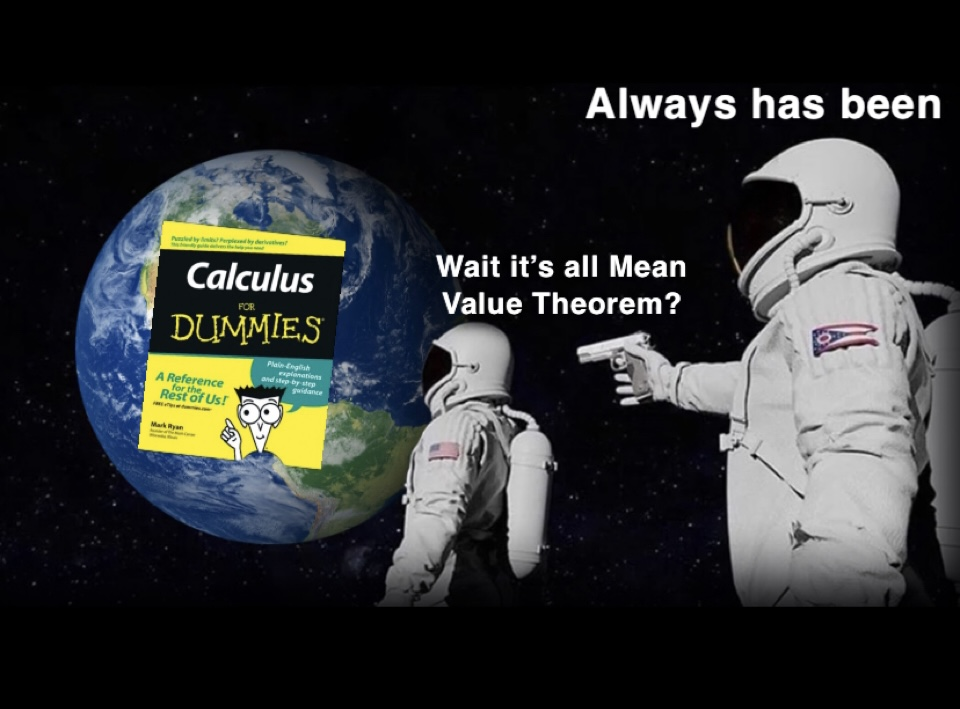
\includegraphics[width=10cm]{IMG_0106.jpg}
    \caption{The cake is a lie.}
    \label{fig:astro}
\end{figure}
\begin{definition}
    Let $f$ be a real function defined on a metric space $X$. We say that $f$ has a \vocab{local maximum} at a point $p\in X$ if there exists $\delta>0$ such that $f(q)\leq f(p)$ for all $q\in X$ with $d(p,q)<\delta$. (Local minima are defined similarly.)
\end{definition}
    
\begin{theorem}
    Let $f$ be defined on $[a,b]$. If $f$ has a local maximum at a point $x\in(a,b)$, and if $f'(x)$ exists, then $f'(x)=0$.
\end{theorem}
\begin{remark}
    To prove, choose $\delta>0$ such that $f(q)\leq f(p)$ for all $p\in X$ with $d(p,q)<\delta$. Then \[a<x-\delta<x<x+\delta<b.\]If $x-\delta<t<x$, then \[\frac{f(t)-f(x)}{t-x}\geq0,\]so as $t\rightarrow x$, $f'(x)\geq0$. If $x<t<x+\delta$, then 
    \[\frac{f(t)-f(x)}{t-x}\leq 0,\]so $f'(x)\leq 0$.
\end{remark}
\begin{theorem}[Generalized Mean Value Theorem]
    If $f$ and $g$ are continuous real functions on $[a,b]$ which are differentiable in $(a,b)$, then there exists a point $x\in (a,b)$ where \[[f(b)-f(a)]g'(x)=[g(b)-g(a)]f'(x).\]
\end{theorem}
\begin{remark}
    Note that differentiability is \textit{not} required at endpoints. To prove, let \[h(t)=[f(b)-f(a)]g(t)-[g(b)-g(a)]f(t)\quad(a\leq t\leq b).\]
    Notice that $h$ is continuous on $[a,b]$, differentiable on $(a,b)$, and \[h(a)=f(b)g(a)-f(a)g(b)=h(b).\]To finish the proof, we need to show $h'(x)=0$ for some $x\in(a,b)$. If $h$ constant, we're done. If $h(t)>h(a)$ for some $t\in(a,b)$, then $h$ attains its maximum at some $x$ on the closed (compact) interval $[a,b]$. Since $h(a)=h(b)$, $x\in(a,b)$. If $h(t)<h(a)$, for some $t\in(a,b)$, the same argument applies to choose an $x$ where $h$ attains its minimum. 
\end{remark}
\begin{theorem}[The Mean Value Theorem]
    If $f$ is a real continuous function on $[a,b]$, which is differentiable in $(a,b)$, then there is a point $x\in(a,b)$ at which \[f(b)-f(a)=(b-a)f'(x).\]
\end{theorem}
\begin{remark}
    The proof follows immediately after taking $g(x)=x$ in the Generalizeed Mean Value Theorem.
\end{remark}
\begin{theorem}
    Suppose $f$ is differentiable in $(a,b)$:
    \begin{enumerate}
        \ii If $f'(x)\geq 0$ for all $x\in(a,b)$, then $f$ is monotonically increasing.
        \ii If $f'(x)=0$ for all $x\in(a,b)$, then $f$ is constant.
        \ii If $f'(x)\leq 0$ for all $x\in(a,b)$, then $f$ is monotonically decreasing.
    \end{enumerate}
\end{theorem}

\subsection{Continuity of Derivatives}
\begin{moral}
    Not every function is a derivative!
\end{moral}
Derivatives which exist at every point in an interval have one important quality that they share with functions continuous on that interval: intermediate values are assumed.
\begin{theorem}
    Suppose $f$ is a real differentiable function on $[a,b]$ and suppose $f'(a)<\lambda<f'(b)$. Then there is a point $x\in(a,b)$ such that $f'(x)=\lambda$. (A similar result holds if $f'(a)>f'(b)$.)
\end{theorem}
\begin{remark}
    To prove, let\[g(t)=f(t)-\lambda t.\]Since $\lambda>f'(a)$, we know $g'(a)<0$ so $g(t_{1})<g(a)$ for some $t_{1}\in(a,b)$. Similarly, $g(t_{2})<g(b)$ for some $t_{2}\in(a,b)$, so $g$ attains minimum on $(a,b)$. Thus there exists some $x\in(a,b)$ such that $g'(x)=0$, and thus $0=f'(x)-\lambda$.
\end{remark}
\begin{corollary}
    If $f$ is differentiable on $[a,b]$, then $f'$ cannot have any simple discontinuities on $[a,b]$. (But may very well have discontinuities of the second type. See the following example)
\end{corollary}
\begin{example}[Deja vu]
    The function \[f(x)=\begin{cases}
        x^{2}\sin(\frac{1}{x}) & x\neq 0,\\
        0 & x=0.
    \end{cases}\]is differentiable but $f'$ is discontinuous a $x=0$.
\end{example}

\subsection{L'Hospital's Rule}
\begin{theorem}
    Suppose $f$ and $g$ are real and differentiable in $(a,b)$ and $g'(x)\neq 0$ for all $x\in (a,b)$, where $-\infty\leq a<b\leq+\infty$. Suppose
    \[\frac{f'(x)}{g'(x)}\rightarrow A\textrm{ as }x\rightarrow a.\]
    If $f(x)\rightarrow 0$ and $g(x)\rightarrow 0$ as $x\rightarrow a$, or if $g(x)\rightarrow+\infty$ as $x\rightarrow a$, then \[\frac{f(x)}{g(x)}\rightarrow A\textrm{ as }x\rightarrow a.\]
\end{theorem}
\begin{remark}
    Like most things in this chapter, you can use the Mean Value Theorem to prove this statement. That being said, I'm running on 2 hours of sleep and have been up for nearly 24 hours straight, so this one's not getting written down here.
\end{remark}
\subsection{Derivatives of Higher Order}
\begin{definition}
    If $f$ has a derivative $f'$ on an interval, and $f'$ itself is differentiable, we denote the derivative of $f'$ by $f''$ and call $f''$ the second derivative of $f$. We can continue in the same manner to obtain \[f,f',f'',f(3),\dotsc,f^{(n)},\]where $f^{(n)}$ is called the $n$th derivative of $f$. In order for $f^{(n)}(x)$ to exist at a point $x$, $f^{(n-1}$ must exist in a neighborhood of $x$, and be differentiable at $x$, and so on...
\end{definition}
\subsection{Taylor's Theorem}
\begin{theorem}
    Suppose $f$ is a real function on $[a,b]$, $n\in\NN$, $f^{(n-1)}$ is continuous on $[a,b]$, and $f^{(n)}(t)$ exists for every $t\in(a,b)$. Let $\alpha,\beta$ be distinct points of $[a,b]$ and define\[P(t)=\sum_{k=0}^{n-1}\frac{f^{(k)}(\alpha)}{k!}(t-\alpha)^{k}.\]Then there exists a point $x$ between $\alpha$ and $\beta$ such that \[f(\beta)=P(\beta)+\frac{f^{(n)}(x)}{n!}(\beta-\alpha)^{n}.\]For $n=1$, this is just the mean value theorem (but are we \textit{that} surprised?)
\end{theorem}
In general, Taylor's Theorem lets us approximate functions with polynomials of degree $n-1$, and (arguably most importantly,) estimate the error if we know bounds on $|f^{(n)}(x)|.$
\begin{remark}
    Again, this uses the Mean Value Theorem in its proof. zzz
\end{remark}
\subsection{Differentiation of Vector-Valued Functions}
\begin{remark}
    In terms of vector valued functions, $\vec{f}(x)$ is the point of $\RR^{k}$ (if there is one) for which
    \[\lim_{t\rightarrow x}\left|\frac{\vec{f}(t)-\vec{f}(x)}{t-x}-\vec{f}'(x)\right|=0,\]and $\vec{f}'$ is again a function with values in $\RR^{k}$. If $f_{1},\dotsc,f_{k}$ are the components of $\vec{f}$, then \[\vec{f}' = (f'_{1},\dotsc,f'_{k}),\]and $\vec{f}$ is differentiable at a point $x$ if, and only if, each of the functions $f_{1},\dotsc,f_{k}$ is differentiable at $x$.
\end{remark}
Unfortunately, the Mean Value Theorem (and thus L'Hopital's Rule) don't necessarily hold in $\RR^{k}$.
\begin{example}[RIP the GOAT: MVT \textit{was} the MVP]
    Let $f(x)=e^{ix}=\cos(x)+i\sin(x).$ Then \[f(2\pi)-f(0)=1-1=0,\]but \[f'(x)=ie^{ix},\](and thus $|f'(x)|=1$ for all $x\in\RR$.)
\end{example}
\begin{example}[French Hospital est trés pauvre]
    On the open interval, define $f(x)=x$ and \[g(x)=x+x^{2}e^{i/x^{2}}.\]Notice that as $x\rightarrow 0$, both $f(x)$ and $g(x)$ approach 0. Since $|e^{it}|=1$ for all $t\in\RR$, notice that
    \[\lim_{x\rightarrow0}\frac{f(x)}{g(x)}=1.\]
    Next, \[g'(x)=1+\left(2x-\frac{2i}{x}\right)e^{i/x^{2}}\quad(0<x<1),\]so that \[|g'(x)|\geq\left|2x-\frac{2i}{x}\right|-1\geq \frac{2}{x}-1.\]Thus \[\left|\frac{f'(x)}{g'(x)}\right|=\frac{1}{|g'(x)|}\leq\frac{x}{2-x}\]so\[\lim_{x\rightarrow0}\frac{f'(x)}{g'(x)}=0.\]
    Repose en paix, mon doux hôpital.
\end{example}
\begin{theorem}[A New Hope]
    Suppose $\vec{f}$ is a continuous mapping of $[a,b]$ into $\RR^{k}$ and $\vec{f}$ is differentiable in $(a,b)$. Then there exists $x\in(a,b)$ such that \[|\vec{f}(b)-\vec{f}(a)|\leq(b-a)|\vec{f}'(x)|.\]
\end{theorem}
\begin{remark}
    Let $\vec{z}=\vec{f}(b)-\vec{f}(a),$ and define 
    \[\phi(t)=\vec{z}\cdot \vec{f}(t)\quad(a\leq t\leq b).\]Then $\phi$ is a real-valued continuous function on $[a,b]$ which is differentiable in $(a,b)$. By the Mean Value Theorem (hooray! it's back!):
    \[\phi(b)-\phi(a)=(b-a)\phi'(x)=(b-a)\vec{z}\cdot\vec{f}'(x)\]for some $x\in(a,b)$. On the other hand, 
    \[\phi(b)-\phi(a)=\vec{z}\cdot\vec{f}(b)-z\cdot\vec{f}(a)=\vec{z}\cdot\vec{z}=|\vec{z}|^{2}.\]Thus,
    \[|\vec{z}|^{2}=(b-a)|\vec{z}\cdot\vec{f}'(x)|\leq(b-a)|\vec{z}||\vec{f}'(x)|,\]so $|\vec{z}|\leq(b-a)|\vec{f}'(x)|$. 
\end{remark}
\newpage
\begin{center}
    
\includegraphics[scale=.1]{cah.jpg}\\[2cm]
\end{center}
\end{document}